% !TEX root = ../thesis-example.tex
%
\chapter{Personal Interaction}
\section{Calibration and Recovery of Personal Pointing Gesture}
\label{section:4-PAST}
%why the topic is coming to important 
It is widely believed that as the computing,communication, and display technologies progress further, the existing user interaction solution may become a bottleneck for the effective interaction with desired information. 
Today, we are facing more and more digital information controlled by different computing devices.
Selection is the first and one of the important steps in the natural user interaction process as the computing device has to know which object the user is interested in. In most cases, the user is aware of where and what the information is but can't directly begin interaction since time is lost to make the corresponding computing device know where the desired information is\cite{Swindells2002}. 
For example, different information can be shown in multiple displays, however, the user will have a problem interacting with the information if the displays are not within reach. In addition, computers can understand the ambient scenario via object detection or 3D reconstruction, but the user can't directly perform interaction with the desired object or tell the computers how to understand the 3D volume\cite{export:244725}.
Hence, designing better natural user interfaces is still an vital concern.

The pointing gesture is fundamental to human behavior \cite{Matthews2012} and used consistently across cultures \cite{McNeill2000}. It begins at an early developmental stage \cite{Carpendale2010} and lets humans  reference proximal objects as well as abstract concepts in the world. It is also natively combined with hand gestures. Pointing gestures, which are part of our gestural language, are inherently used for interaction\cite{Nanayakkara2013a}. Only a few works try to model and estimate the user{\rq}s pointing geometry when performing interaction with ambient information.One existing technique consists in positioning a camera next to the monitor or display and observing the user. In this case, the computing device can understand the user{\rq}s pointing behavior by detecting the user{\rq}s gaze. Unfortunately, the user has to stand within a limited working zone defined by the targeted display and the camera, as shown in \figurename{ \ref{fig:4-PAST:problem}(a)}.
Other inventors have taken advantage of wearable cameras enabling the user to perform interaction with digital information\cite{Harrison2011} \cite{Mistry2009}.
These works detect the user's finger and calculate the pointing geometry from the camera view instead of the user's eye, as shown in \figurename{ \ref{fig:4-PAST:problem}(b)}. This setup works well when the user performs interaction with information which should is reachable.
%The camera view still could replace the user view when a visual hint was display or the user's view is controlled.
However, \figurename{ \ref{fig:4-PAST:problem}(c)} illustrates an important problem when the user equipped with a wearable camera tries to point at objects which are not reachable. There is a significant offset between $O_{eye}$, the object which is pointed towards in the user's view, and $O_{camera}$, the object in the camera's view. 
\begin{figure} [htb]
	\centering
	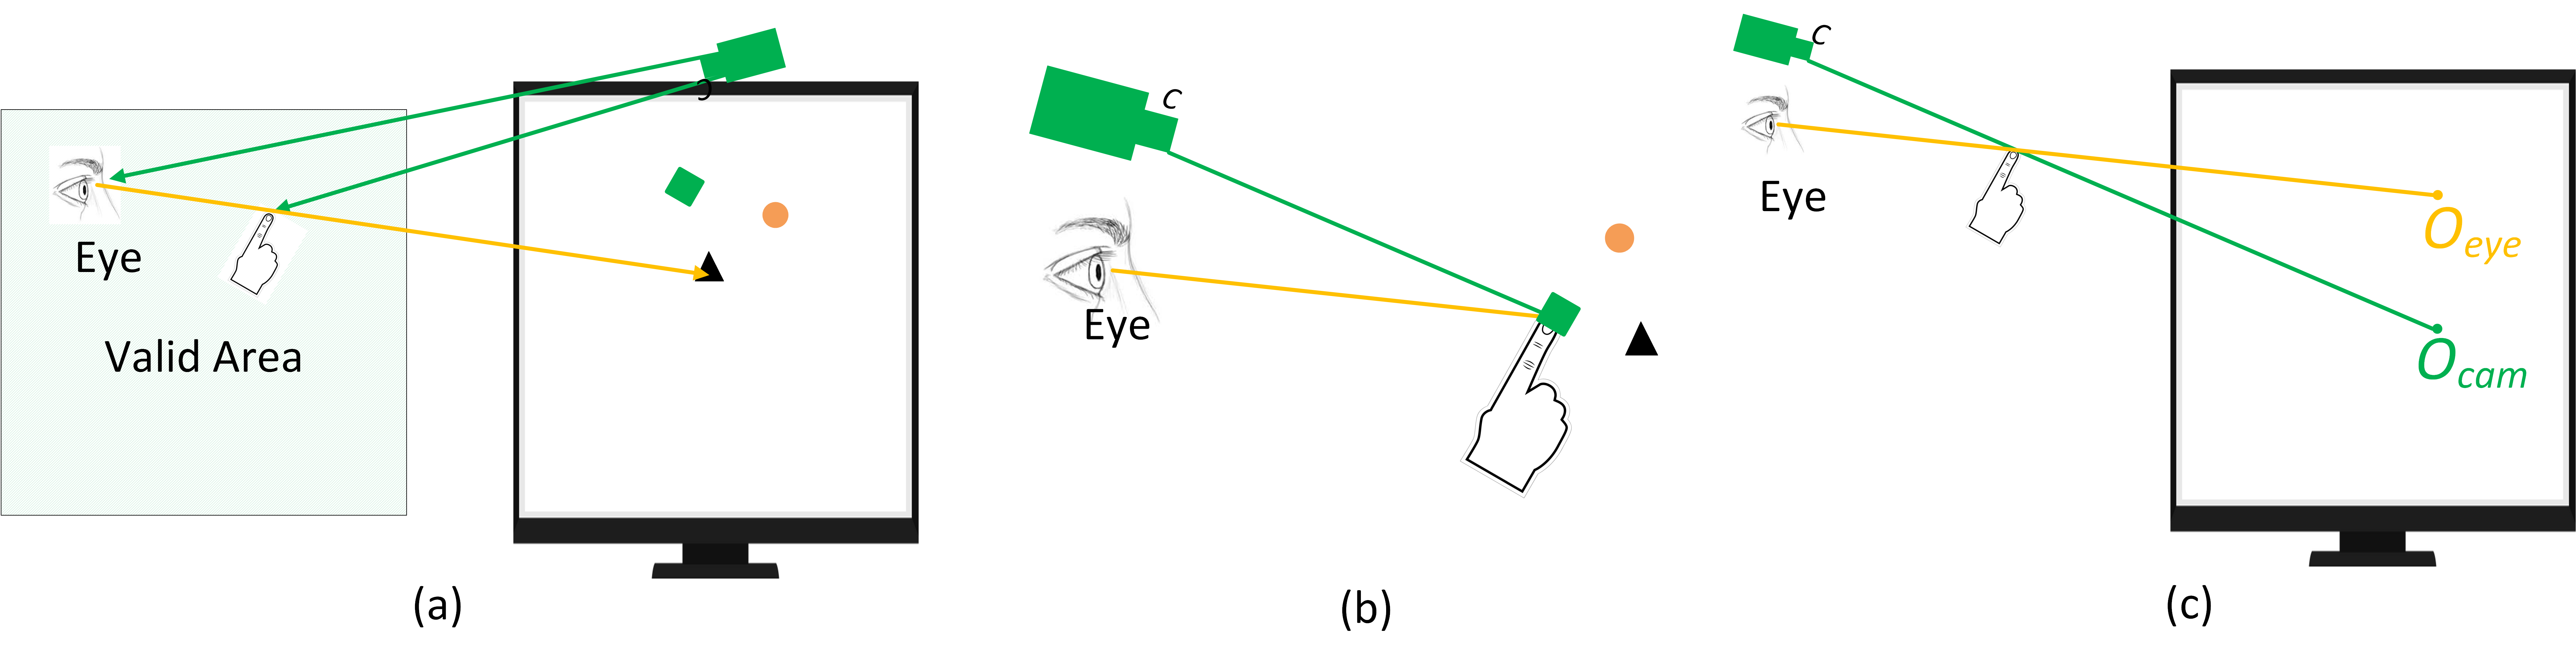
\includegraphics[width= 1.0\linewidth]{figures/4-PAST/problem.png}
	\caption{(a)There is a limited working zone, when positioning a camera next to the monitor or display while observing the user.(b)The user's view could be replaced by the camera view when the desired object is reachable. (c) There is a significant offset when the user points at a not reachable object.}
	\label{fig:4-PAST:problem}
\end{figure}
Wearable vision systems have potential ability to acquire contextual information through computer vision techniques\cite{Kurata2000}. Usually, the wearable device calibration is not possible and often scale, rotation, and/or translation-invariant features are required in higher level modules. If the wearable device could understand the user{\rq}s pointing geometry, then the pointing gesture will augment the capabilities of the wearable device by enabling a multi-point control 3D interface in a mixed reality (MR) setting. Here we aim at developing  an ubiquitous solution allowing the wearable device to always understand the spatial relationship between the user{\rq}s specific pointing gesture and the ambient information within the mixed reality world.

\subsection{PAST Methodology}
\label{sec:4-PAST:Methodology}
we propose a method that facilitates a wearable device calibration of a user's pointing gesture in order to model and recover the user specific pointing geometry. The pointing geometry is modeled as a line of sight, which starts from a virtual eye center and goes through the fingertip to the desired target information. During the calibration process, the user is asked to perform pointing gestures towards several targets shown to them. A user specific virtual eye center is then estimated based on the detected fingertip.
This process enables to accurately determine where the user is pointing at in a mixed reality environment. This work is different than the current methods for hand gesture recognition and gesture based interaction.  Its main difference lies within a novel concept and method for calibrating and recovering the pointing geometry with a user's specific habit, enabling direct interaction with real and virtual digital elements of interest within the user's environment.

\subsubsection{General Design}
\label{sec:4-PAST:GD}
In a general hardware design, the wearable device should be put on the user's head and contain two sensors, $S_{f}$ and $S_{c}$. The  $S_f$ is used to detect the fingertip which the user uses to perform the pointing gesture and calculate its 3D position. The $S_c$ goes to acquire the contextual information of the objects in front of the user. In general, the  $S_f$ should provide a near-range depth map as the 3D position of the fingertip has to be accurately calculated. The contextual information should be acquired with 3D position as the pointing gesture is performed in the 3D world.The $S_c$ could be a color camera, a depth sensor or a RGB-D sensor in different scenarios to acquire a known object with 3D position or a valid depth map of the real world. The $S_c$ could also be calibrated related to a head mounted display (HMD) to acquire the contextual information of the virtual world. As $S_c$ and  $S_f$ are just different types of camera, the self calibration of the wearable device could be performed using Zhang{\rq}s method \cite{Zhang2000}.

\subsubsection{Pointing At Several Targets (PAST)} \label{sec:4-PAST:PAST}
As a human, both eyes perceive a stereo view and the images are processed by our brains to generate the 3D scene of the objects in front of us. We always perceive a unified 3D scene no matter how we rotate our eyes. In other words, there should be a fixed original point of the 3D scene in our brain and here we define it as the virtual eye center. When performing pointing gestures, a user could always directly put their fingertips somewhere between their eyes and the target to generate a line of sight, which goes through the fingertip and the target. Thus we model the pointing geometry as a line, which starts from the virtual eye center and goes through the fingertip and the target, as shown in \figurename{ \ref{fig:4-PAST:PSATCalibration}}. It is important to emphasize that the virtual eye center is not the middle point between the user's eyes. As discussed in Section \ref{sec:4-PAST:results}, users may be left or right eye dominant which affects the location of the virtual eye center. Fortunately, the PAST method accounts for this.

%Inspired by the Single-Point Active Alignment Method (SPAAM) for Optical See-Through head mounted display calibration for augmented reality \cite{Tuceryan2000},
The objective of \textbf{Pointing At Several Targets (PAST)} method is to calibrate and recover the specific pointing geometry. The result of the calibration is the position of a virtual eye center $E$ for the user. Based on the pointing model, we could collect a set of pointing lines and estimate the intersection to finish the calibration.
As shown in \figurename{ \ref{fig:4-PAST:PSATCalibration}}, the target ,$T_i$, is shown somewhere at the front of the user, who is asked to perform a pointing gesture towards $T_i$ using one finger naturally. The 3D positions of the fingertips $F_i$ and $T_i$ are collected through $S_f$ and $S_c$, respectively. The pointing line $L_i$ ,which passes through $F_i$ and $T_i$, would also go through $E$ . After enough pointing lines are collected, the intersection of the lines should be $E$. After calibration, the user specific virtual eye-center $E$ is known and the pointing geometry would be recovered as $L_{i}$, going through $E$ and  $F_i$, when the pointing gesture is performed.
\begin{figure} [htb]
	\centering
	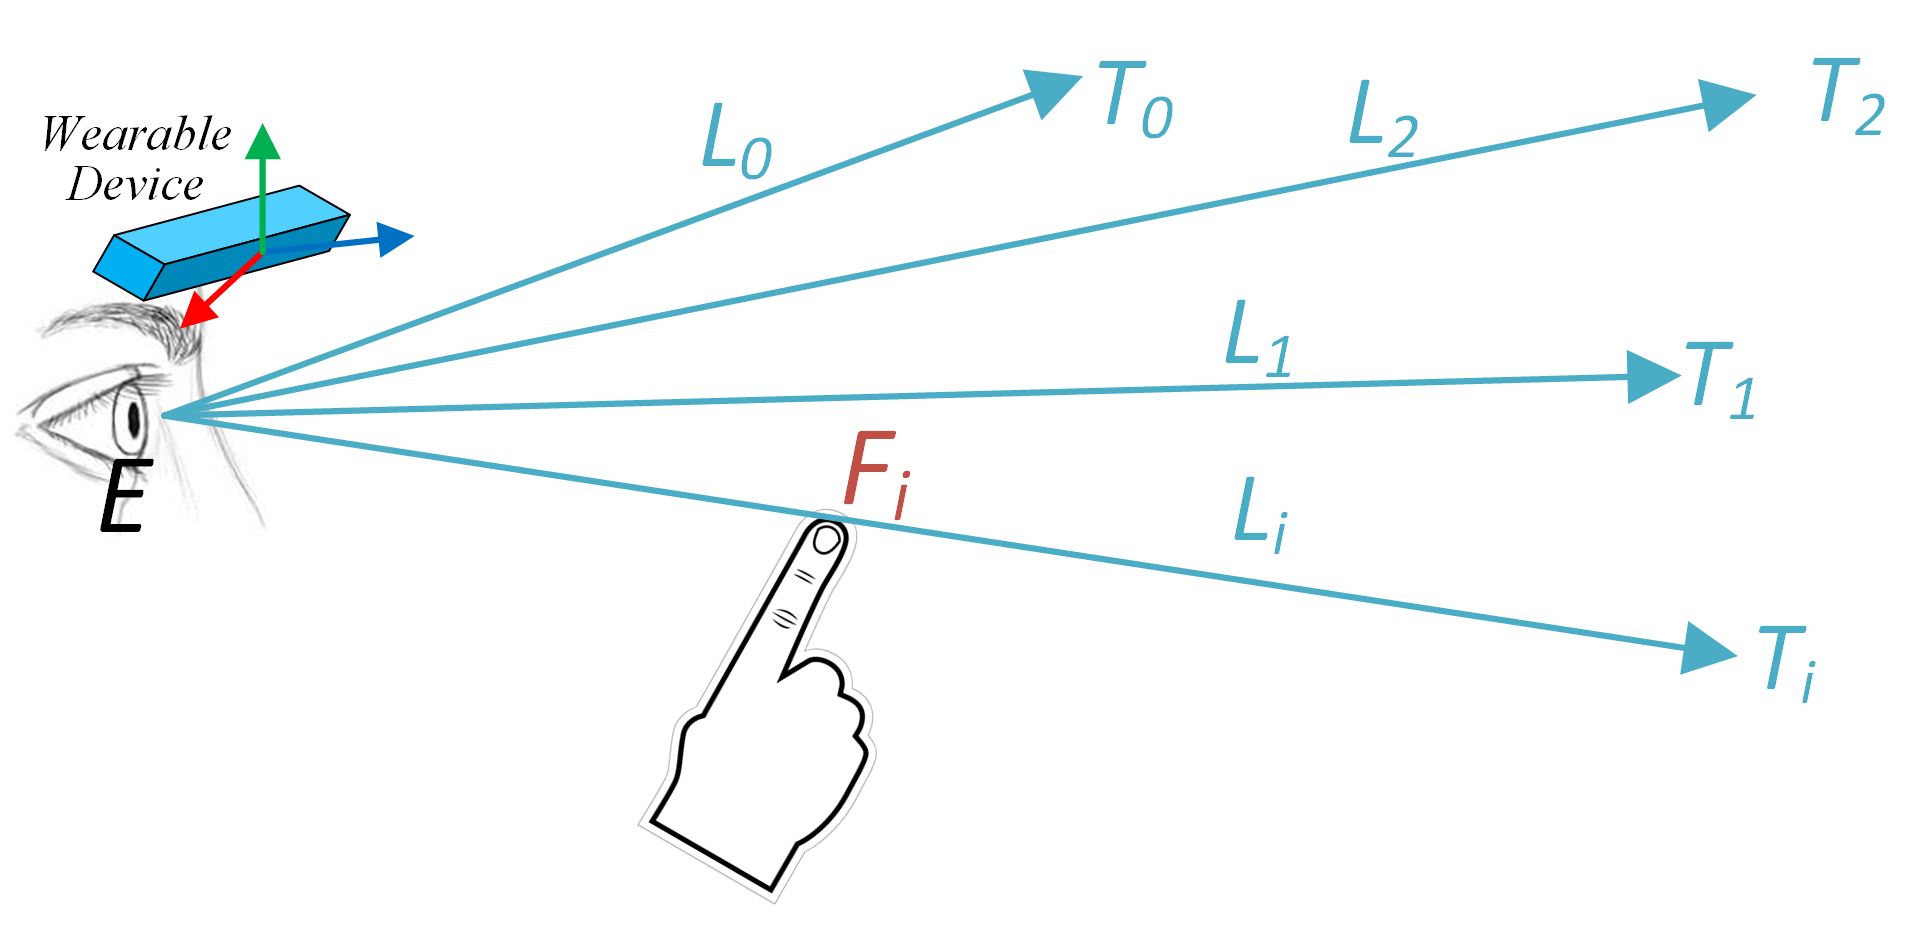
\includegraphics[width= \linewidth]{figures/4-PAST/Calibration.png}
	\caption{Calibration of the user specific pointing gesture: the user is asked to point at several targets using one finger and the pointing lines which pass through $F_i$ and $T_i$ are collected. The intersubsection of these lines should be $E$, the user specific virtual eye-center.}
	\label{fig:4-PAST:PSATCalibration}
\end{figure}

\subsubsection{Target the user points at} \label{sec:4-PAST:findTarget}
As defined in section \ref{sec:4-PAST:GD}, the contextual information always could be expressed in a 3D world and a mesh surface could be generated accordingly. 
Based on the PAST method, the user specific pointing geometry could be recovered as the pointing line $L_{i}$, going through $E$ and  $F_i$, when the pointing gesture is performed.
As shown in \figurename{ \ref{fig:4-PAST:pointToTarget}} , a $Mesh$ surface is generated based on the contextual information. The intersection between $L_{i}$ and $Mesh$ is $T_i$, the target which the user points at. 
\begin{figure} [htb]
	\centering
	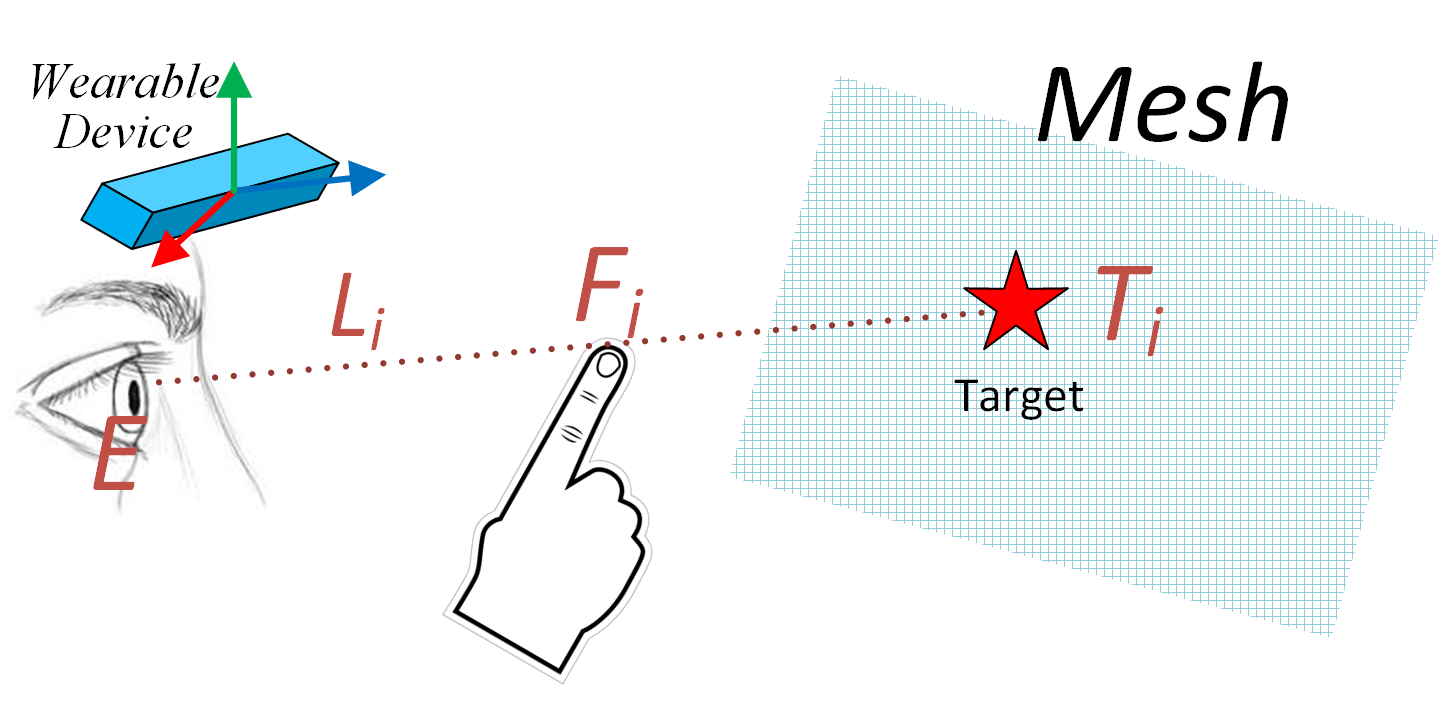
\includegraphics[width= \linewidth]{figures/4-PAST/pointToTarget.png}
	\caption{ The intersection between the pointing line $L_{i}$ and the $Mesh$ is  $T_i$, the 3D position of the target or information the user points at.}
	\label{fig:4-PAST:pointToTarget}
\end{figure}

We propose an example scenario where the user is equipped with a wearable RGB-D sensor to perform a pointing gesture interaction with information shown on a display.
The depth sensor generates a near-range depth map and acts as $S_f$, and the color camera as $S_c$ acquires the contextual information. The 3D position of a fingertip could be calculated from a valid depth map when the pointing gesture is performed. It is very easy to detect a display and compute its plane function using image features. As the targets are shown on the display, the 3D contextual information of the display and the targets are acquired using the color camera. The calibration of the RGB-D sensor is performed using Zhang{\rq}s method \cite{Zhang2000}. During the PAST calibration, the targets are shown on the display and the user is asked to perform pointing gesture towards the targets (see Section \ref{sec:4-PAST:PAST}). After calibration, the pointing line $L_i$ is calculated and the  $Mesh$ is generated from the plane function of the display. According to \figurename{ \ref{fig:4-PAST:pointToTarget}}, the intersection between the pointing line $L_{i}$ and $Mesh$ is  $T_i$, the 3D position of the target or information shown on the display the user is pointing at.

\subsection{Feasibility Analysis of PAST} \label{sec:4-PAST:FA}
The pointing gesture is fundamental to human behavior and is also quite personal \cite{Matthews2012}. If the images in the user's eyes were accessible, then $F_i$ , the fingertip detected in $S_f$, and $E$, the eye center calculated in PAST calibration, would be perfect. In addition, the human eyes are an auto-focus stereo camera, but can't focus on objects in different depths at the same time. In our proposed system, the user is asked to focus on the target and not on the fingertip, which allows the user to perform the pointing naturally. Thus the fingertip in the user's view is different from the one detected by $S_f$. 

As shown in \figurename{ \ref{fig:4-PAST:fingertipOffset}}, $F_i$  and $T_i$  are the fingertip and the target, which are detected by the wearable device respectively, and $E$ is the virtual eye center calculated in the PAST calibration procedure. $\bar F_i$ and $\bar T_i$ are the fingertip and target in the user{\rq}s own view, and $\bar E$ is the ideal virtual eye center. So there is a vector $V_{fi}$ from $\bar F_i$ to $F_i$, $F_i = {\bar F_i} + V_{fi}$ when the pointing is performed at all times. $T_i = {\bar T_i}$ in the calibration procedure as the user is asked to point towards a known target. $L_i$ is the pointing line estimated by the wearable device and $\bar L_i$ is the ideal pointing line in the user{\rq}s view. 
\begin{figure} [htb]
	\centering
	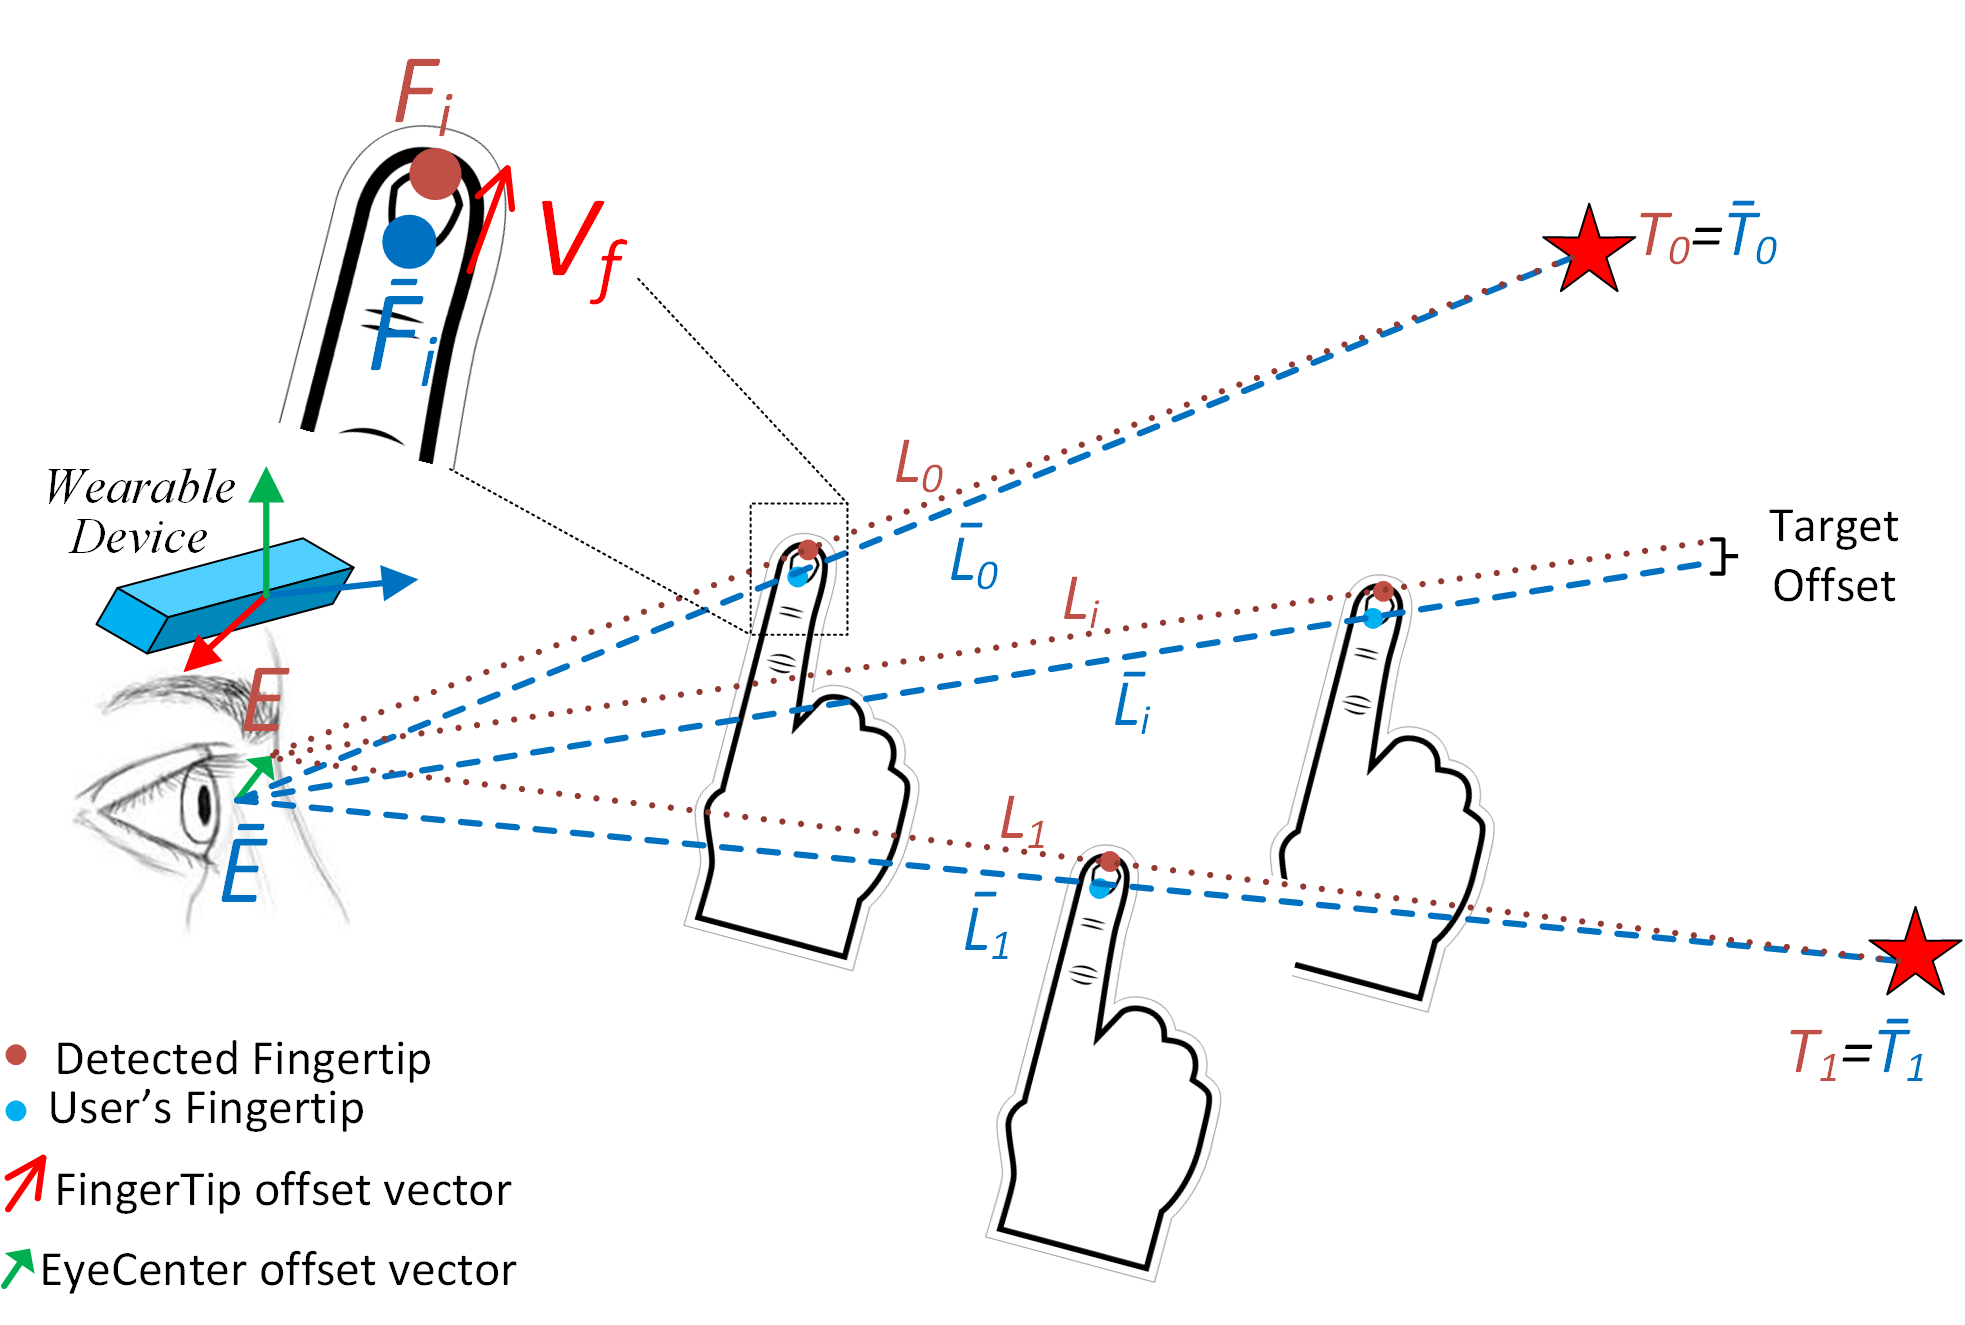
\includegraphics[width= \linewidth]{figures/4-PAST/fingerOffset.png}
	\caption{ Here is the pointing geometry during the calibration and recovery procedure. There is a vector $V_{fi}$  from $\bar F_i$ to $F_i$ when the pointing gesture is performed and a vector $V_{E}$, from the ideal virtual eye-center ${\bar E}$ to $E$.}
	\label{fig:4-PAST:fingertipOffset}
\end{figure}
\subsubsection{Calibration} \label{sec:4-PAST:PASTCalibration}
Based on the assumption of the pointing geometry model, the pointing line $\bar L_i$ is starting from $\bar E$ going through $\bar F_i$ and ending at the desired target $\bar T_i$. We could use Eq. \ref{equ:pointOnLineUser} to  represent all the points along the pointing line $\bar L_i$, and $\bar E$ is the intersection of all the pointing line $\bar L_i$. This means that there is a $\bar \lambda_i$ making both Eq.\ref{equ:lambdaLineuser} and Eq.\ref{equ:intersectionOfLineUser} true for every  $\bar L_i$.
\begin{equation}  \label{equ:pointOnLineUser}
P_{\bar L_i} = {\bar T_i} + \bar\lambda ({\bar F_i} - {\bar T_i}) ,\bar\lambda \in R 
\end{equation}
\begin{equation} \label{equ:lambdaLineuser}
\bar\lambda_i = \frac {D_{\bar E2 \bar T_i}}{D_{\bar E2 \bar T_i} -D_{\bar E2 \bar F_i}} 
\end{equation}
where $D_{\bar E2 \bar F_i}$ is the distance from $\bar E$ to ${{\bar F_i}}$ and $D_{\bar E2 \bar T_i}$ is the distance from ${\bar E}$ to ${\bar T_i}$. 
\begin{equation} \label{equ:intersectionOfLineUser}
{\bar E} = {\bar T_i} + \bar\lambda_i ({\bar F_i} - {\bar T_i}) 
\end{equation}
The pointing line detected by the wearable device is $L_i$, which goes through  ${T_i}$ and $F_i$. All the points along $L_i$ could be represented as:
\begin{equation} \label{equ:pointOnLineSensor}
P_{L_i} = {T_i} + \lambda(F_i - {T_i}) , \lambda \in R 
\end{equation}
$F_i$ in Eq. \ref{equ:pointOnLineSensor} could be replaced by ${\bar F_i} + V_{fi}$ and ${T_i} = {\bar T_i}$ during calibration. Hence,
\begin{equation} \label{equ:pointOnlineSensor2}
P_{L_i} = {\bar T_i} + \lambda({\bar F_i} - {\bar T_i}) + \lambda V_{fi}, \lambda \in R 
\end{equation}
There is a point $E_i$ on the line $P_{L_i}$, when $\lambda = \bar\lambda_i$ in Eq.\ref{equ:pointOnlineSensor2}.
\begin{equation} \label{equ:P_eye}
E_i = {\bar T_i} + \bar\lambda_i({\bar F_i} - {\bar T_i}) + \bar\lambda_i V_{fi}  
\end{equation}
After putting Eq. \ref{equ:intersectionOfLineUser} into Eq.\ref{equ:P_eye}, there is always a point $E_i$ along every $L_i$ and could be represent as:
\begin{equation} \label{equ:P_eye2}
E_i = {\bar E} + \bar\lambda_i V_{fi}  
\end{equation}
\begin{figure} [htb]
	\centering
	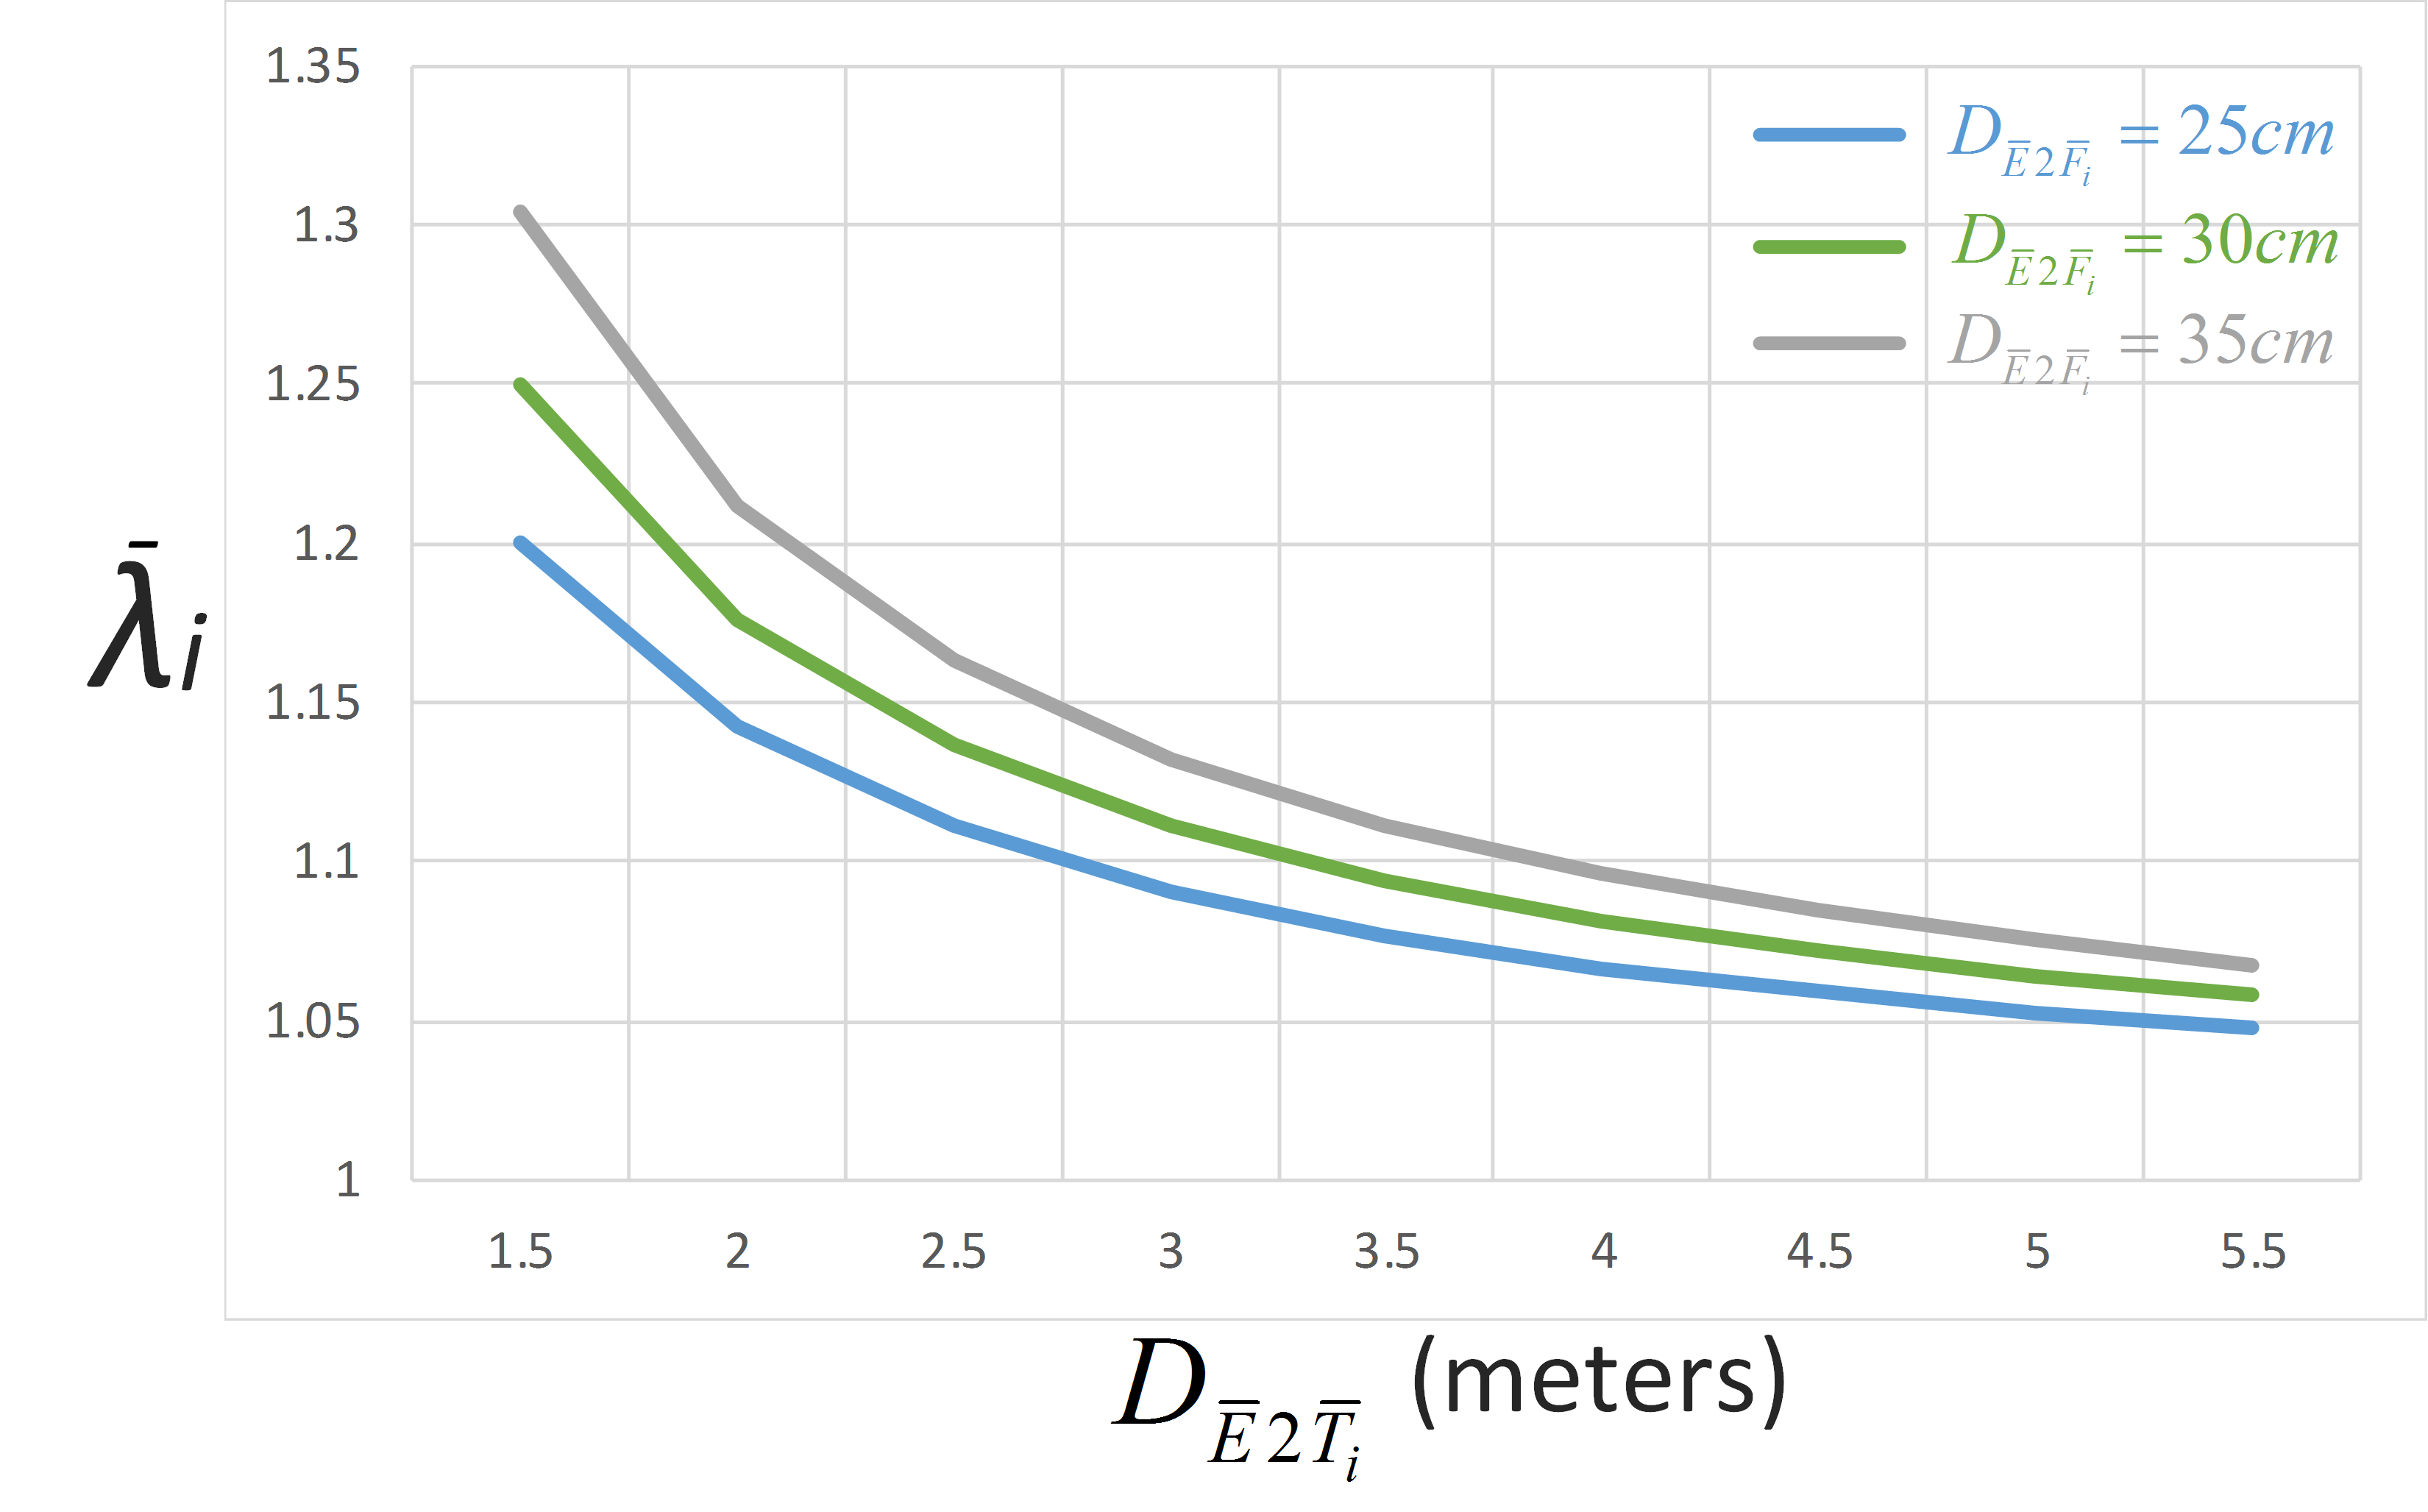
\includegraphics[width= \linewidth]{figures/4-PAST/lambdai.png}
	\caption{$\bar \lambda_i$ decreases as $D_{\bar E2 \bar T_i}$ increases in three different cases, but the difference is very small.}
	\label{fig:4-PAST:lambdai}
\end{figure}
%and the maximum length of  $V_{fi}$  is about the size of nail, 10 mm
When PAST calibration is performed, we could fix the $D_{\bar E2 \bar T_i}$ and $\bar \lambda_i$ is only affected by $ D_{\bar E2 \bar F_i}$. As shown in \figurename{ \ref{fig:4-PAST:lambdai}}, $\bar \lambda_i$ decreases slowly as $D_{\bar E2 \bar T_i}$ increases in three different example cases. The maximum delta of $\bar \lambda_i$ is smaller than 0.1. $\bar\lambda_i$ could be rewritten as:
\begin{equation} \label{equ:lambdai}
\bar\lambda_i = \bar\lambda_c + \Delta \bar\lambda_i
\end{equation}
where $\bar\lambda_c \in \left[1.0,1.2\right]$ is constant part and $\Delta \bar\lambda_i \in \left[0,0.1\right] $. 
$V_{fi}$ is different every time and could also be represented as $V_{fc} + {\Delta V_{fi}}$, where $V_{fc}$ is a stable offset and ${\Delta V_{fi}}$ is a small random deviation. So,
\begin{equation} \label{equ:lambdavf}
\bar\lambda_i V_{fi} \approx  \bar\lambda_c V_{fc}  + \bar\lambda_i {\Delta V_{fi}} %+ \Delta \bar\lambda_i V_{fc} + \bar\lambda_c {\Delta V_{fi}}
\end{equation}
where $\bar\lambda_c {\Delta V_{fi}} + \bar\lambda_i {\Delta V_{fi}}$ is very small.  $\bar\lambda_c V_{fc}$ is consistent, so $\delta \bar\lambda_{i} V_{fc}$ is the main contribution of the variation of $\bar\lambda_i V_{fi}$. Even when there is about 2 cm offset between $F$ and $\bar{F}$, there exist two points $E_m$ and $E_n$ along any two lines $L_m$ and $L_n$ respectively and the maximal distance between $E_m$ and $E_n$ is about 0.2 cm. There is a valid candidate point $E$, which is very close to of all the lines $L_i$. Hence, the PAST calibration is feasible and the offset between $E$ and $\bar{E}$ is approximately $ \bar\lambda_c V_{fc}$. 
\begin{equation} \label{equ:P_eyeCalib}
E \approx {\bar E} + \bar\lambda_c V_{fc} 
\end{equation} 
\subsubsection{Pointing geometry recovery} \label{sec:4-PAST:PASTrecovery}
As shown in \figurename{ \ref{fig:4-PAST:fingertipOffset}}, $E$ is the calibration result with an offset $V_{E} \approx \bar\lambda_c V_{fc}$, between $E$ and the ideal virtual eye-center ${\bar E}$. 
When the user points towards a target after calibration, the position of the target calculated by the wearable device, $T_i$, could be represented by $E$ and $F_i$ as:
\begin{equation} \label{equ:targetInSensor}
T_i = E+ \frac{D_{E2T_i}}{D_{E2F_i}}  \left( {F_i - E} \right)
\end{equation}
where $D_{E2F_i}$ is the distance from $E$ to ${{F_i}}$ and $D_{E2T_i}$ is the distance from ${E}$ to ${T_i}$. \\
$\bar T_i$ , the position of the ideal target in the user's view, could be expressed as:
\begin{equation} \label{equ:targetInEye}
\bar T_i \approx {\bar E} + \frac{D_{E2T_i}}{D_{E2F_i}}  \left( {{\bar F_i} - {\bar E}} \right)
\end{equation}
${\angle}_{E}$, the angle error between the user's pointing lines to $T_i$ and $\bar T_i$ could be calculated using Eq.\ref{equ:tanViewAngle} as $D_{E2T_i}$ is much larger than the offset of the target. 
\begin{equation} \label{equ:tanViewAngle}
{\angle}_{E} = \tan^{-1} \left( {\frac{| {T_i - \bar T_i}| }{D_{E2T_i}} } \right)
\end{equation}
After substituting Eq.\ref{equ:P_eyeCalib}, Eq.\ref{equ:targetInSensor} and Eq.\ref{equ:targetInEye}, we get :
\begin{equation} \label{equ:tanViewAngle1}
{\angle}_{E} \approx \tan^{-1} \left( {{\frac{{\lambda_c{|V_{fc}|} }}{D_{E2T_i}} + \frac{{|\lambda_i V_{fi} - \lambda_c V_{fc}|} }{D_{E2F_i}}} } \right)
\end{equation}
As ${\angle}_{E}$ is very small, we get after substituting Eq.\ref{equ:lambdavf}:
\begin{equation} \label{equ:ViewAngleError}
{\angle}_{E} \approx \frac{ {\lambda_c{|V_{fc}|}} }{D_{E2T_i}} + \frac{ {|\Delta \bar \lambda_i V_{fc}|} }{D_{E2F_i}}
\end{equation}
\begin{figure} [htb]
	\centering
	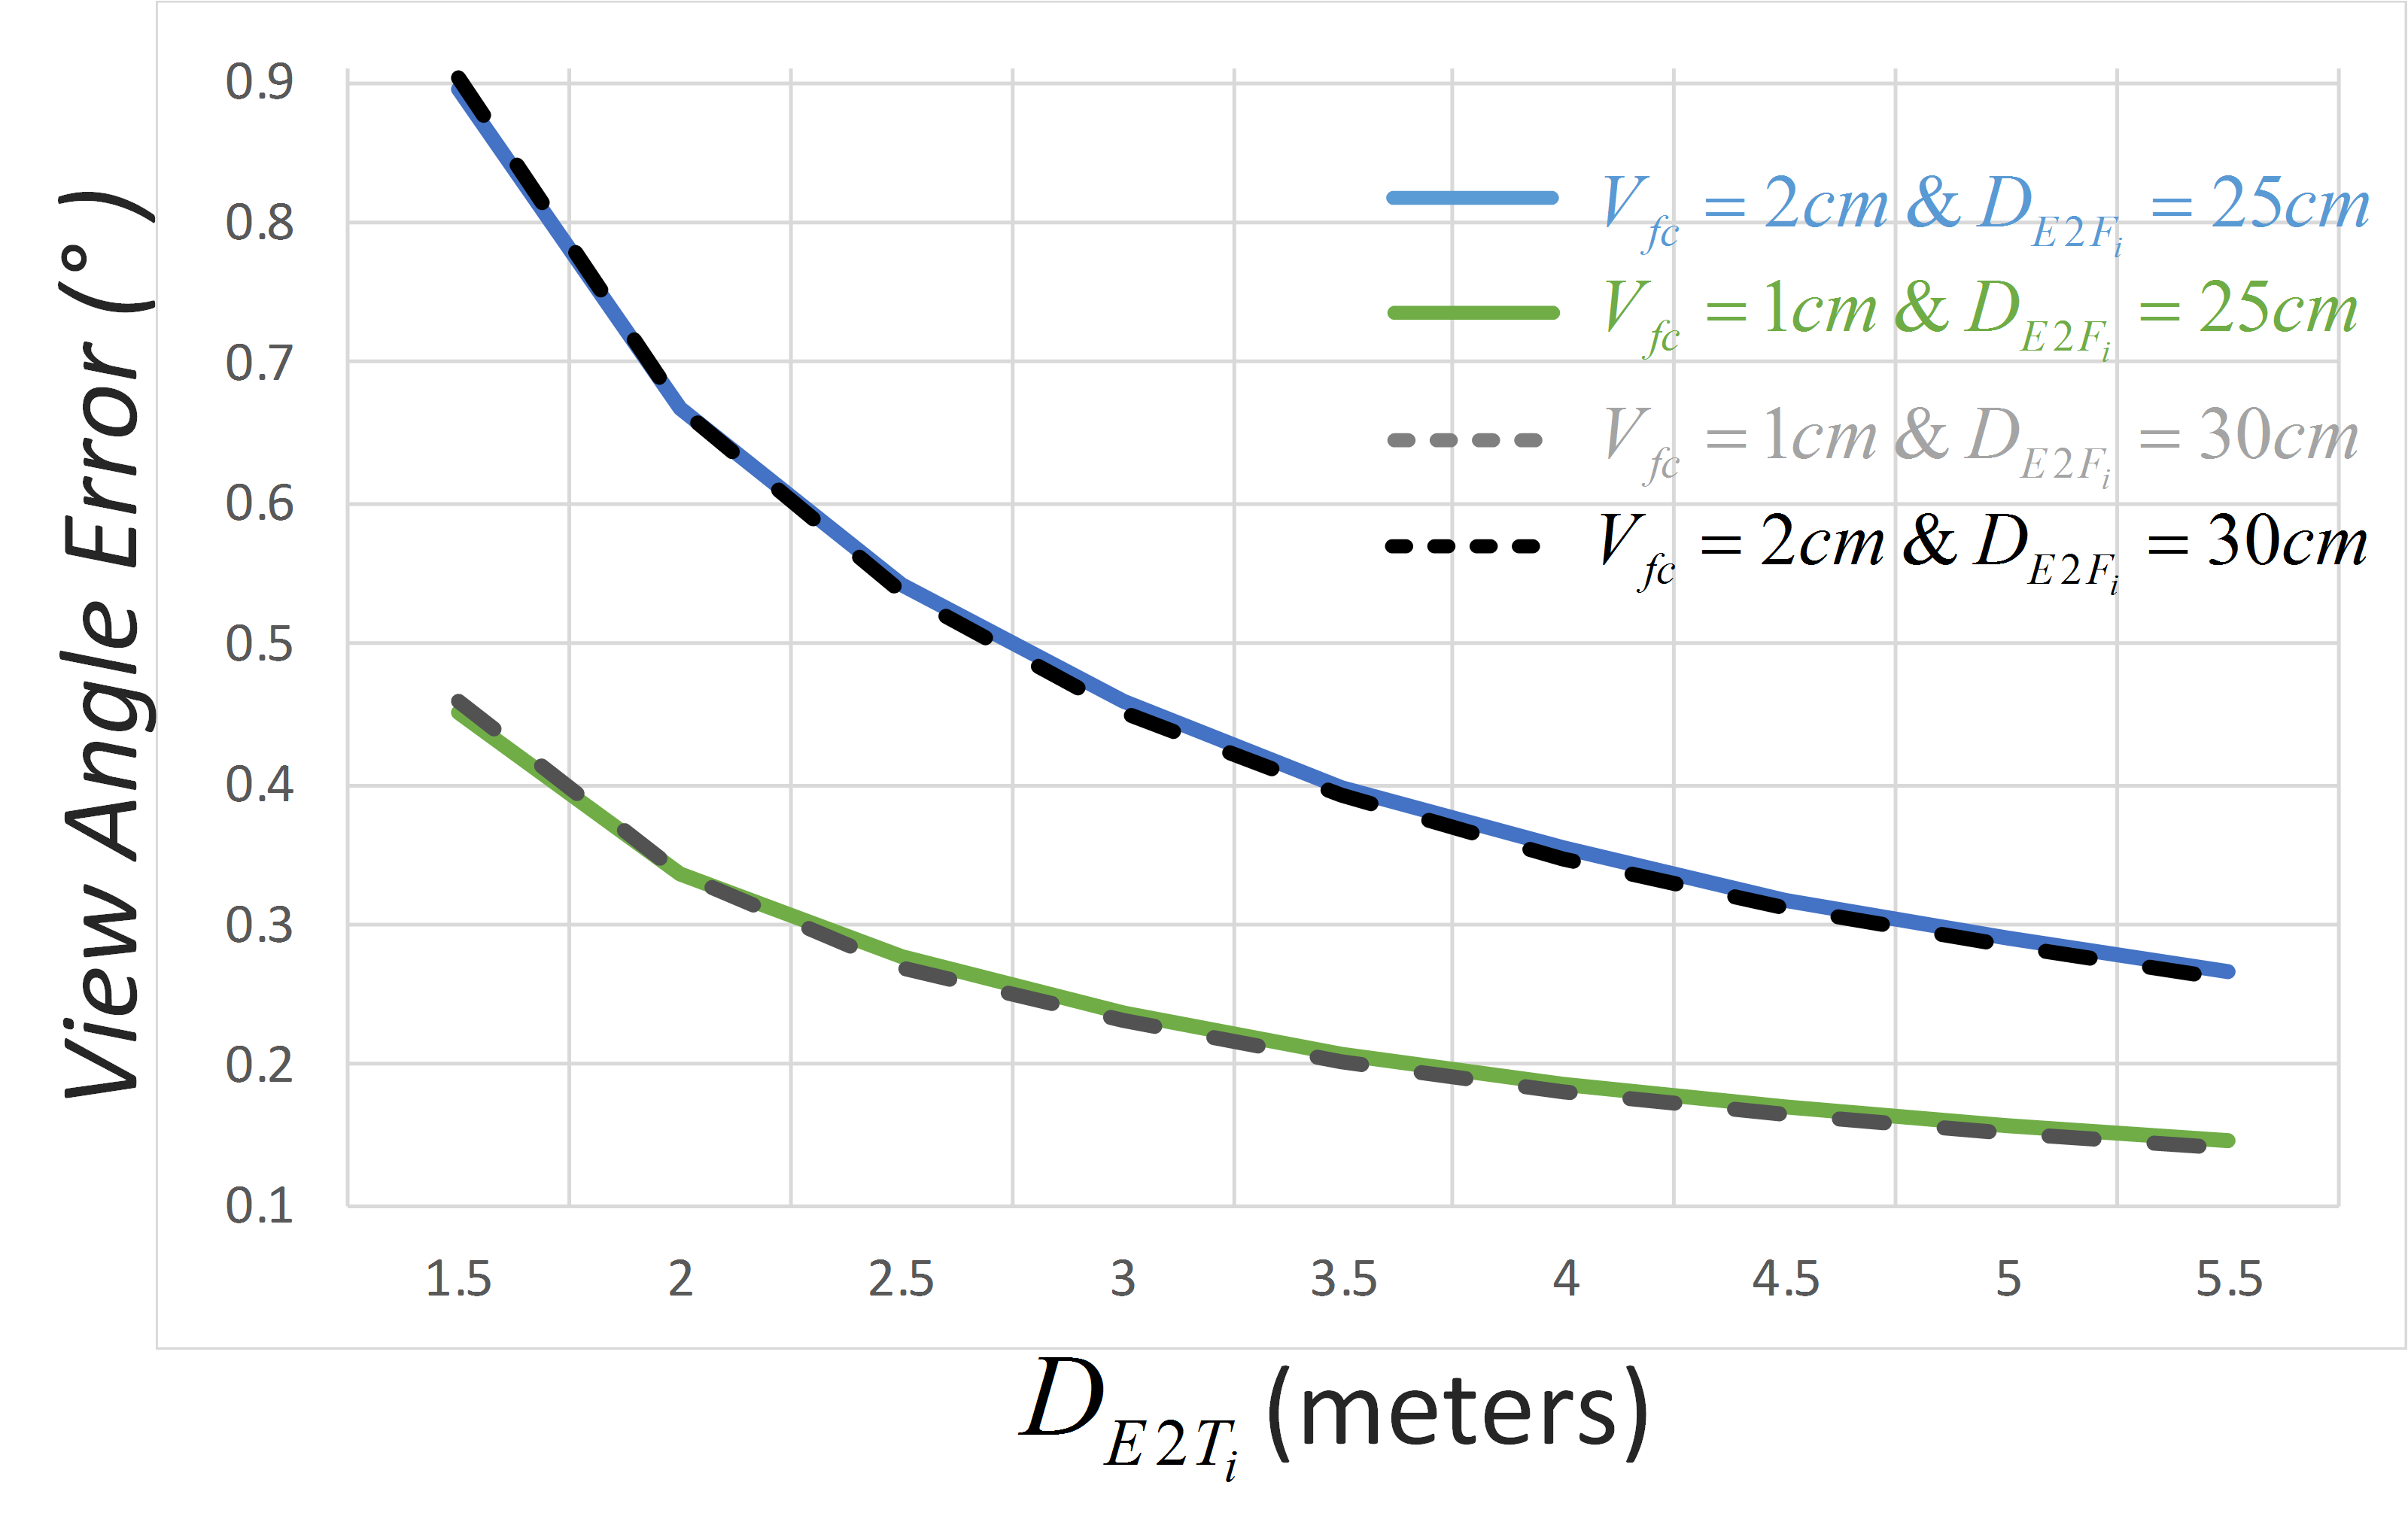
\includegraphics[width= \linewidth]{figures/4-PAST/EvaluationOfPointing.png}
	\caption{The angle error decreases as $D_{E2T}$ increases and $V_{fc}$ decreases. $D_{E2F}$ does not really affect the accuracy of the pointing gesture.}
	\label{fig:4-PAST:evaluatinOfPointing}
\end{figure}
As shown in \figurename{ \ref{fig:4-PAST:evaluatinOfPointing}}, the angle error decreases as $V_{fc}$ decreases and $D_{E2T_i}$ increases. $D_{E2Fi}$ does not really affect the accuracy of the recovered pointing gesture. The accuracy of recovered pointing line is below 0.9\degree.

Based on the above feasibility analysis we can conclude that the PAST method recovers a user specific virtual eye center which enables the wearable device to determine where the user points at accurately.

\subsection{Evaluation \& Results}
%todo: pointing evaluation with one eye to make sure that the method is correct in the most simple scenario.
\subsubsection{Implementation}
In this part, we implement the example scenario described in section \ref{sec:4-PAST:findTarget}, where the user is equipped with a wearable RGB-D device to perform interaction with a display using pointing gesture.
\paragraph{Hardware}
Intel{\rq}s \textit{RealSense} 3D sensor  was selected to act as the wearable RGB-D device, which contains a 640x480 depth sensor (Valid Range:0.2-1.2 meters) and a 1920x1080 color camera. The depth sensor $S_f$ is used to detect the fingertip  and the color camera $S_c$ to acquire 3D contextual information. The \textit{RealSense} 3D sensor is strapped on the user{\rq}s head using a bandana with an adjusted height and angle (see \figurename{ \ref{fig:4-PAST:hardWare}}). 
A 46$''$ TV display and a 24$''$ monitor were positioned around the user with various information displayed on the screens as the contextual environment. 
%new finger with a raised finger TODO: retake a pircure of the hardware setup
\begin{figure}[htb]
	\centering
	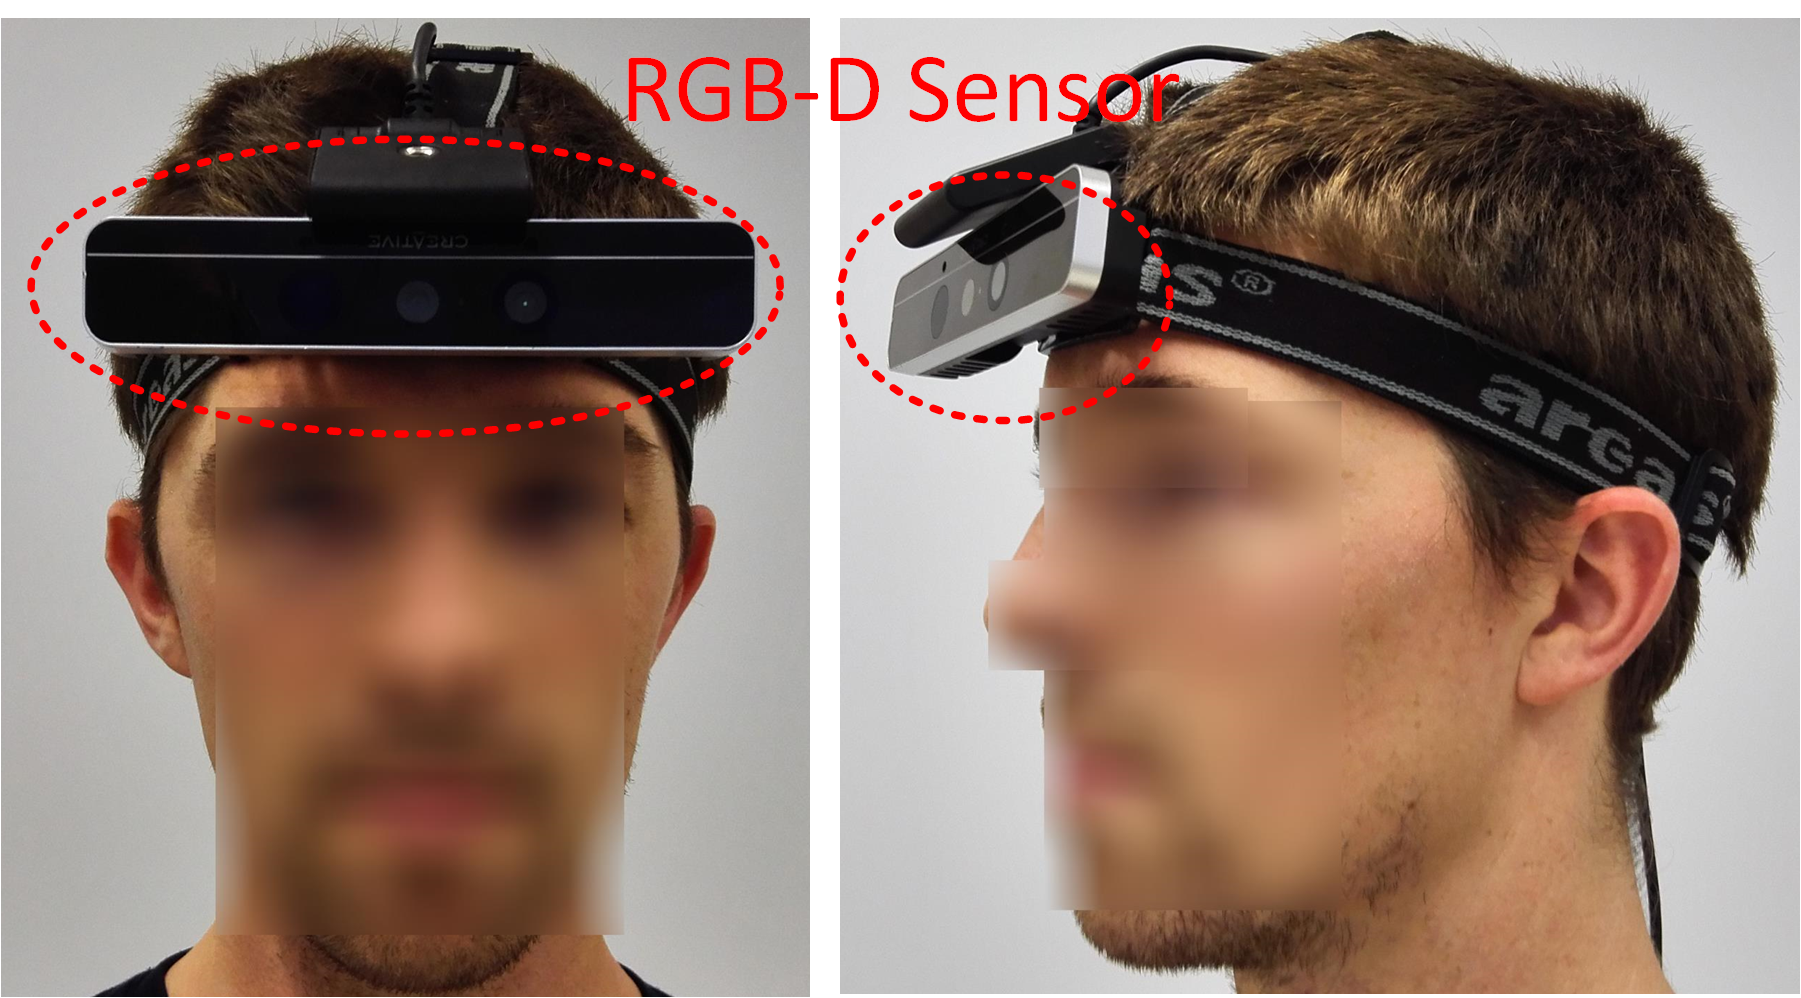
\includegraphics[width = \linewidth]{figures/4-PAST/hardWare.png}
	\caption{The side and front view of the wearable device setup. The \textit{RealSense} 3D sensor is strapped on the user{\rq}s head using a bandana.}
	\label{fig:4-PAST:hardWare}
\end{figure}
\paragraph{Fingertip detection}
%The depth sensor and the color camera are packaged in one device and observe at the same direction. This resulted in not obtaining good contextual information and finger depth maps simultaneously. 
The near range depth sensor could generate a real-time depth image of the hand or finger when the user performs pointing gesture. The fingertip detection technology in \cite{Betancourt2015} was not employed as there was no full depth map of the hand. Hand and finger blobs were directly extracted from the depth image using the \textit{Intel RealSense SDK} and the contours and the convex hull were calculated using the method provided by \cite{Suzuki1985}. Then, the best peak was chosen as the detected fingertip. 
%\textcolor{red}{the following paragraph is not very clear}
%For each fingertip defect, there are 3 points: two peaks and the defect, as shown in \figurename{ \ref{fig:tips}} . We detect a fingertip in the first peak if the angle between the two peaks and the defect is lower than 90\degree and if the norm in pixel is higher than 15.
%\begin{figure} [h]
%	\centering
%	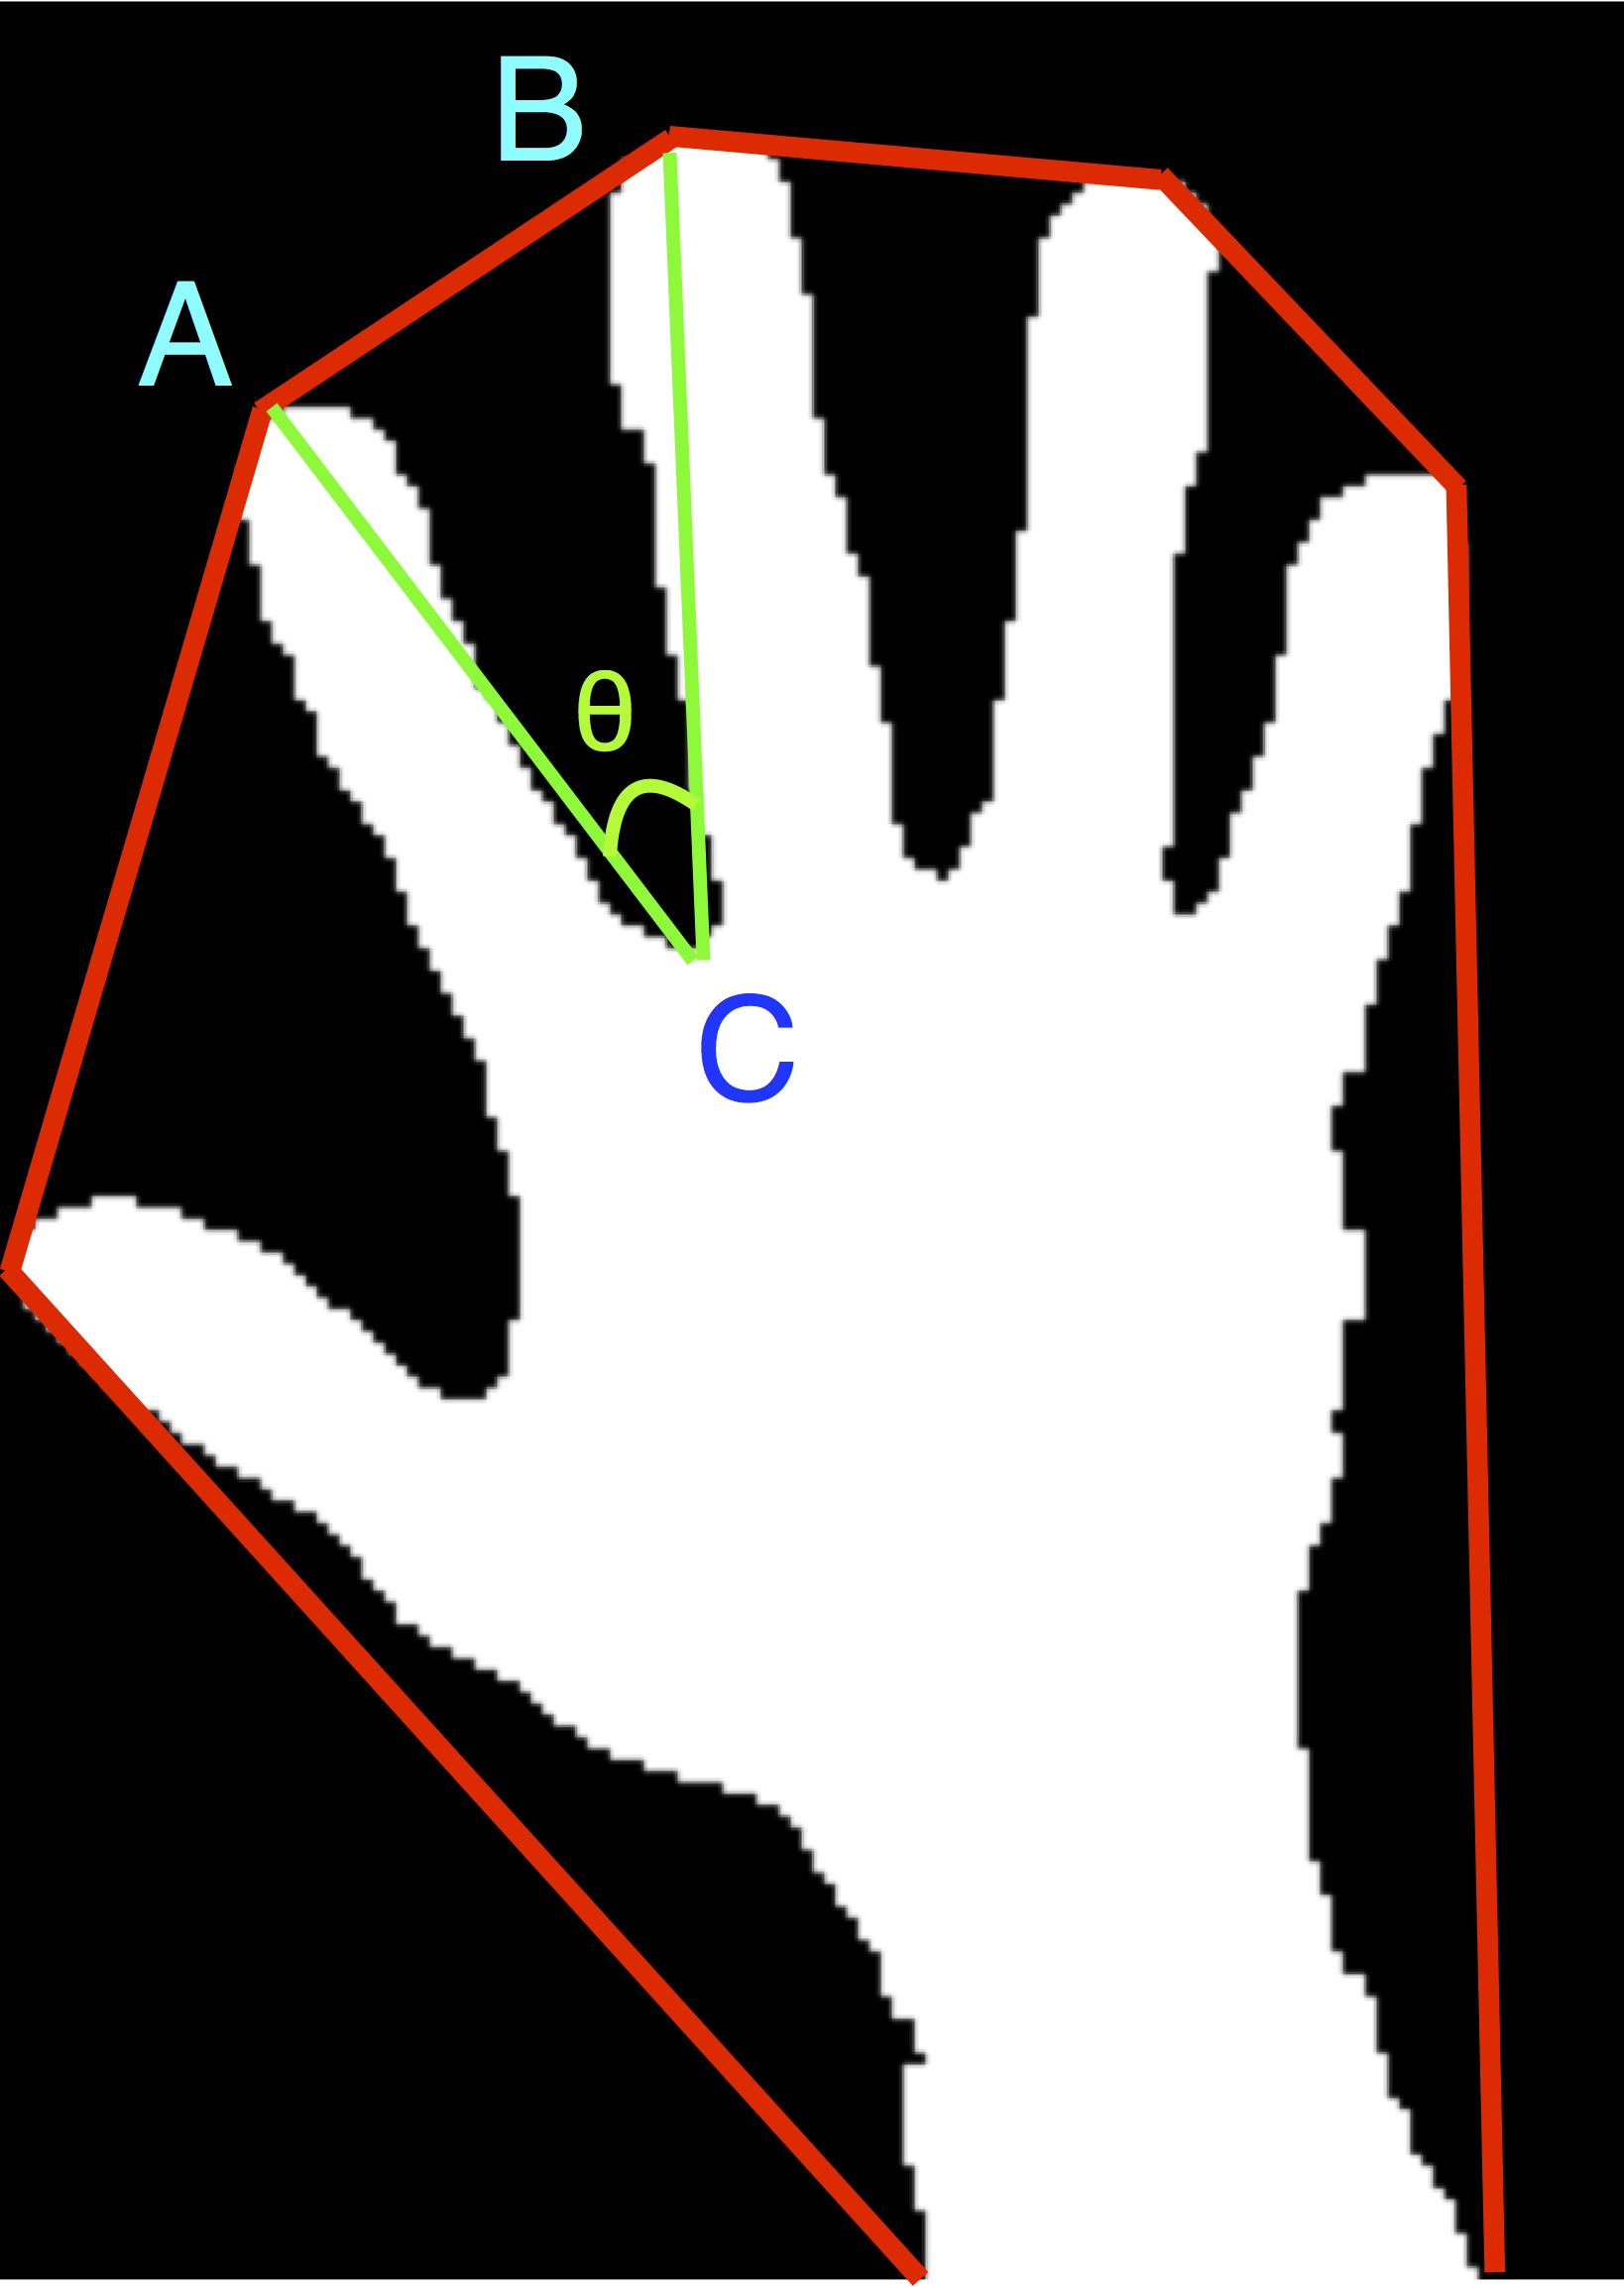
\includegraphics[width=1.5in]{./../images/tips.jpg}
%	\caption {  We detect a fingertip in the first peak if the angle between the two peaks and the defect is lower than 90\degree and if the norm in pixel is higher than 15.}
%	\label{fig:tips}
%\end{figure}
\paragraph{Contextual Information} {\label{sec:4-PAST:markerDetection}}
To simplify the task to acquire the contextual information, we used the \textit{ARTooKitPlus}\cite{Wagner2007a} library to detect the TV display and monitor. There were two implementations: A) Some markers were directly shown  on screen only if it did not affect the current information shown on the screen. The markers instead of the screen were detected to calculate the 3D contextual information. B) Physical printed markers were put next to the display and others were shown on the screen and then a calibration was done to calculate the transformation matrix from the printed markers to the screen. During the user study, the wearable device detected the printed markers and calculated the position of the screen to acquire the contextual information. As shown in \figurename{ \ref{fig:4-PAST:MarkerTracking}}, the screen was detected using method A during the PAST calibration and evaluation and method B was employed during the ``PictureView" demo.
\begin{figure}[htb]
	\centering
	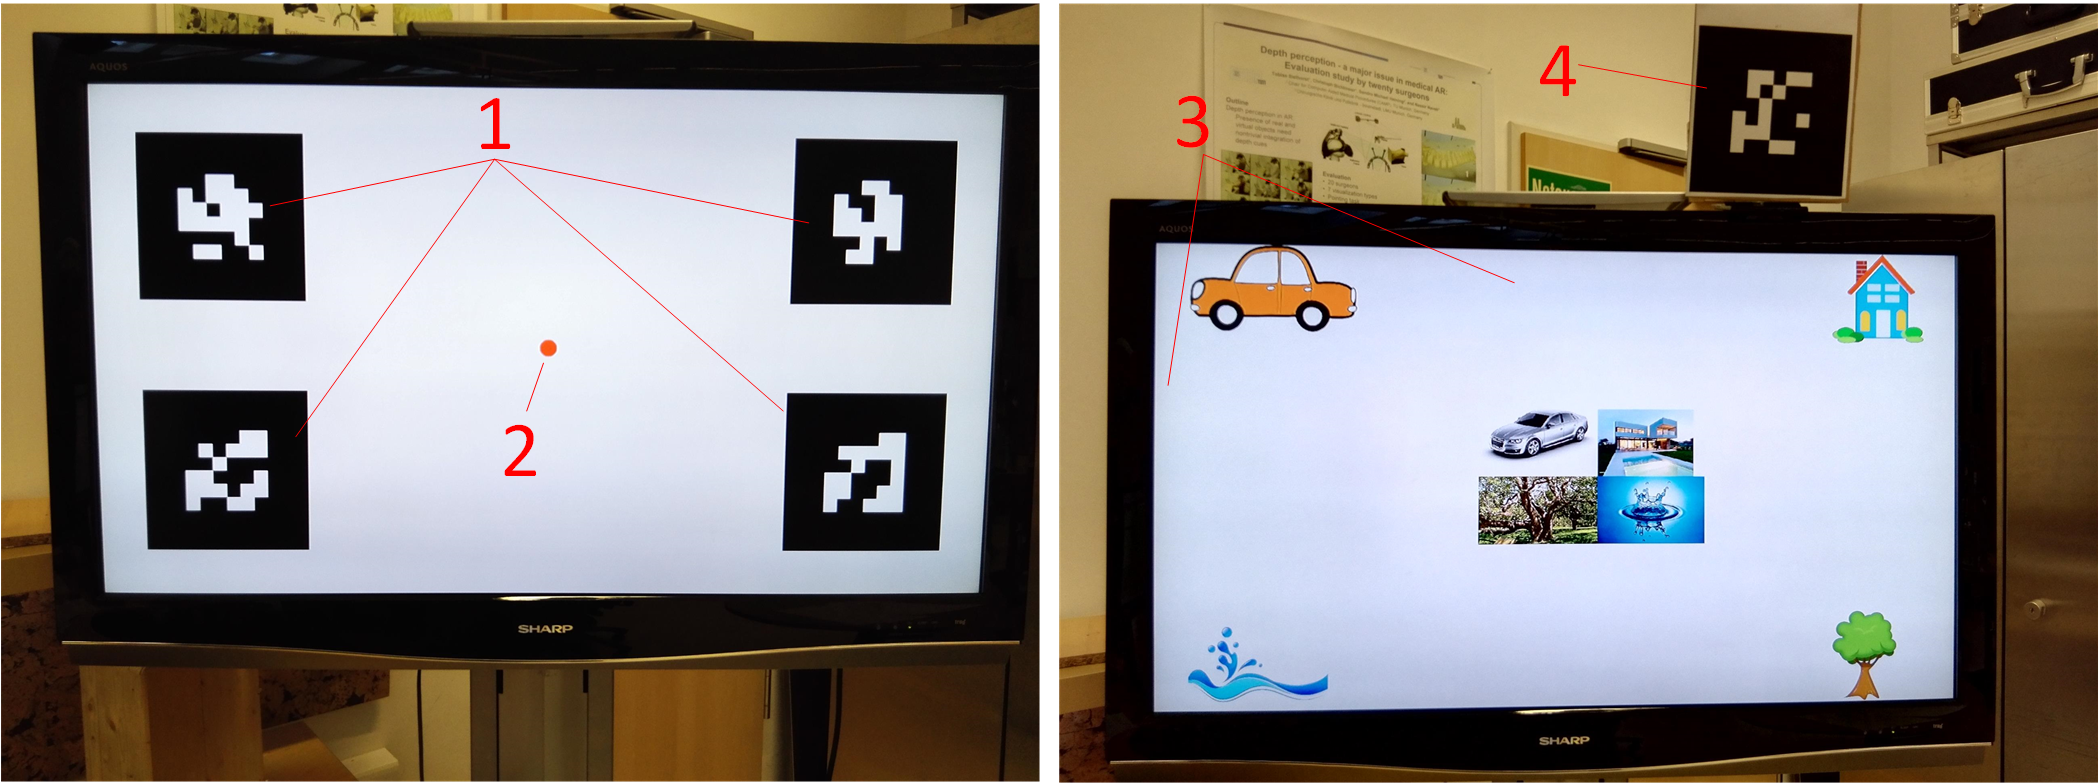
\includegraphics[width = \linewidth]{figures/4-PAST/display.png}
	\caption{(1) Four \textit{ARTooKitPlus} markers shown on the dispaly, (2) A target shown during the PAST calibration, (3) The ``PictureView" demo, (4) A printed \textit{ARTooKitPlus} marker. Left: During the PAST calibration, the screen was detected via the screen marker. Right: A printed marker was tracking during the ``PictureView" demo.}
	\label{fig:4-PAST:MarkerTracking}
\end{figure}
%todo: detection finger tip from two hand at the same time 
%	 how to describe the algorithm to simulate the mouse click 
%	 simple drawing demo using two hands at the same time
\paragraph{PictureView Demo} \label{sec:4-PAST:pictureviewDemo}
In this section, a ``PictureView" demo was developed using the pointing gesture to perform interaction. Several pictures were shown on the screen and the user was asked to select the picture and move it to a defined location, as shown in \figurename{ \ref{fig:4-PAST:MarkerTracking}}. After PAST calibration, the user could directly perform pointing gesture towards the screen to manipulate the picture as the wearable device could recover the pointing geometry and understand the spatial relationship between the pointing gesture and the pictures shown on the display. The selection command was recognized when the user pushed the fingertip along the pointing line. After selection, the picture was moved along the user's pointing gesture. When the picture was moved to the right area, the picture was dissociated with the pointing gesture and disappeared. Or the picture was also dissociated and reset to original position when moved to wrong area. See the supplementary video accompanying this paper.

\subsubsection{User Study Design}
%questions: do we have to keep the first bared-hand cablibration 
To understand the performance and system usability of the PAST method, we conducted some quantitative and qualitative evaluations. For the user study, we designed several tasks in different scenarios and the participants were asked to finish all these tasks. Lastly the users answered a questionnaire to evaluate the ``PictureView" demo.
\paragraph{Scenario for Experiments}
The TV display and the monitor were placed in front of the user. The participant firstly put the wearable RGB-D device on their heads and adjusted the height and angle to make sure that the color camera has a full view of the display in front of them, while ensuring the depth sensor has a valid depth map of the fingertip when they performed pointing gesture in a comfortable pose. There were three kinds of tasks for the user to do during the user study:
\begin{enumerate} [label= (\Alph*)]%[(a)] ,leftmargin=*
	%Evaluation of Calibration method: time consuming and error
	\item \label{task:calib} Calibration: A red target was shown at several different position on the TV display and the user was asked to perform pointing gesture towards the red target using one finger. 
	%The data is automatically collected when the user hold the finger still for one second.
	\item \label{task:pointEvaluation}Evaluation: A blue target was shown at several different position on the TV or the monitor and the user was asked to perform pointing gesture towards the blue target using one finger.
	\item \label{task:PointWithFeedback}Evaluation with visual feedback: A blue target was shown at some different position one the TV. The user performed pointing gesture towards the display with a green point shown as a visual feedback. The user was asked to match the green point and the blue target as close as possible. 
\end{enumerate}
\paragraph{Study Description}
\textbf{Participants}
Ten people (6 Male and 4 Female, and Age Range: 22-34) from different cultures were enrolled in the user study. Three of them were born and brought up in Germany, three in China, two in Chile, one in France and one in India. Seven of them had a degree of computer science. Nine were reported to be right-handed, while one was ambidextrous.

\textbf{Study procedure} Before starting the user study, participants were supervised to perform the pointing in the proposed pose to make sure the wearable device could detect the markers and the fingertip accurately at the same time. The user was asked to focus on the target not the fingertip when performing pointing. After a simple training session, participants were asked to do the following 10 steps to evaluate the proposed method and system.
\begin{enumerate}%[(1)]
	\item \label{step:stereoCalib} Do task \ref{task:calib} three times from 2 meters away to finish PAST calibration and evaluate if the calibration was stable. The first calibration result is employed for all the following evaluation.
	\item \label{step:pointWithFeedback} Do task \ref{task:PointWithFeedback} on the TV display from 2 meters away to give the participant an intuitive feeling of this technology, check the calibration result, and evaluate if the visual feedback would improve the accuracy and precision.
	\item \label{step:pointingEvaluation} Do task \ref{task:pointEvaluation} on the TV display from 2 meters away to evaluate the accuracy and precision of the recovered pointing geometry.
	\item \label{step:diffentHand} Do task \ref{task:pointEvaluation} on the TV display using another hand from 2 meters away to evaluate if the PAST calibration was independent of the finger.
	%one calibration: test with different hand and finger
	\item \label{step:distanceEvaluation} Redo task \ref{task:pointEvaluation} on the TV display from 1.5,3 and 4  meters away, to evaluate the accuracy of the recovered pointing geometry at different distances.
	\item \label{step:differentScreenEvaluation}  Do task \ref{task:pointEvaluation} on the monitor from 2 meters away to evaluate if the calibration is independent of the display.
	\item \label{step:calibDifferentDistance} Redo task \ref{task:calib} three times from 1.5, 3 and 4 meters away to evaluate if the calibration is independent of the target distance. 
	\item \label{step:calibOneEye} Redo task \ref{task:calib} with only left or right eye open from 2 meters away to understand the relationship of the two eyes and the calculated virtual eye center. 
	\item \label{step:pictureview} Play with the demo ``PicureView" for 2 minutes using the first calibration result calculated in step \ref{step:stereoCalib} to evaluate the system usability,.
	\item \label{step:questionnaire} The interpupillary distance of the participant was measured with a ruler and the user completed a questionnaire to evaluate the system.
\end{enumerate}

\subsubsection{Results} \label{sec:4-PAST:results}
%diagrams and analyze the collected data
The real interpupillary distance of the ten participants was measured in step \ref{step:questionnaire} and was distributed from 6.0 to 6.8cm. In step \ref{step:calibOneEye}, the left and right eye were calibrated related to the wearable device and the interpupillary distance was subsequently calibrated. Compared to the true measured distance from step 10, the average distance between eyes is $0.11\pm0.11$ cm. From this, we conclude that the PAST method could accurately measure the user's eye center. 

From step \ref{step:stereoCalib} and \ref{step:calibOneEye}, we could get the positions of the left, right and virtual eye-center related to the wearable device. When all interpupillary distances were upscaled to 7 cm, the spatial relationship of the left, right and virtual eye-center can be seen in \figurename{ \ref{fig:4-PAST:virtualEye}}. 
The position of the virtual eye-center was very user specific and influenced by the user specific pointing gesture. As such, we could not simply take the left eye, right eye, or middle point between the user's eyes as the virtual eye center to recover the pointing geometry. Hence, the PAST calibration is necessary to recover an accurate pointing geometry.
\begin{figure}[htb] 
	\centering
	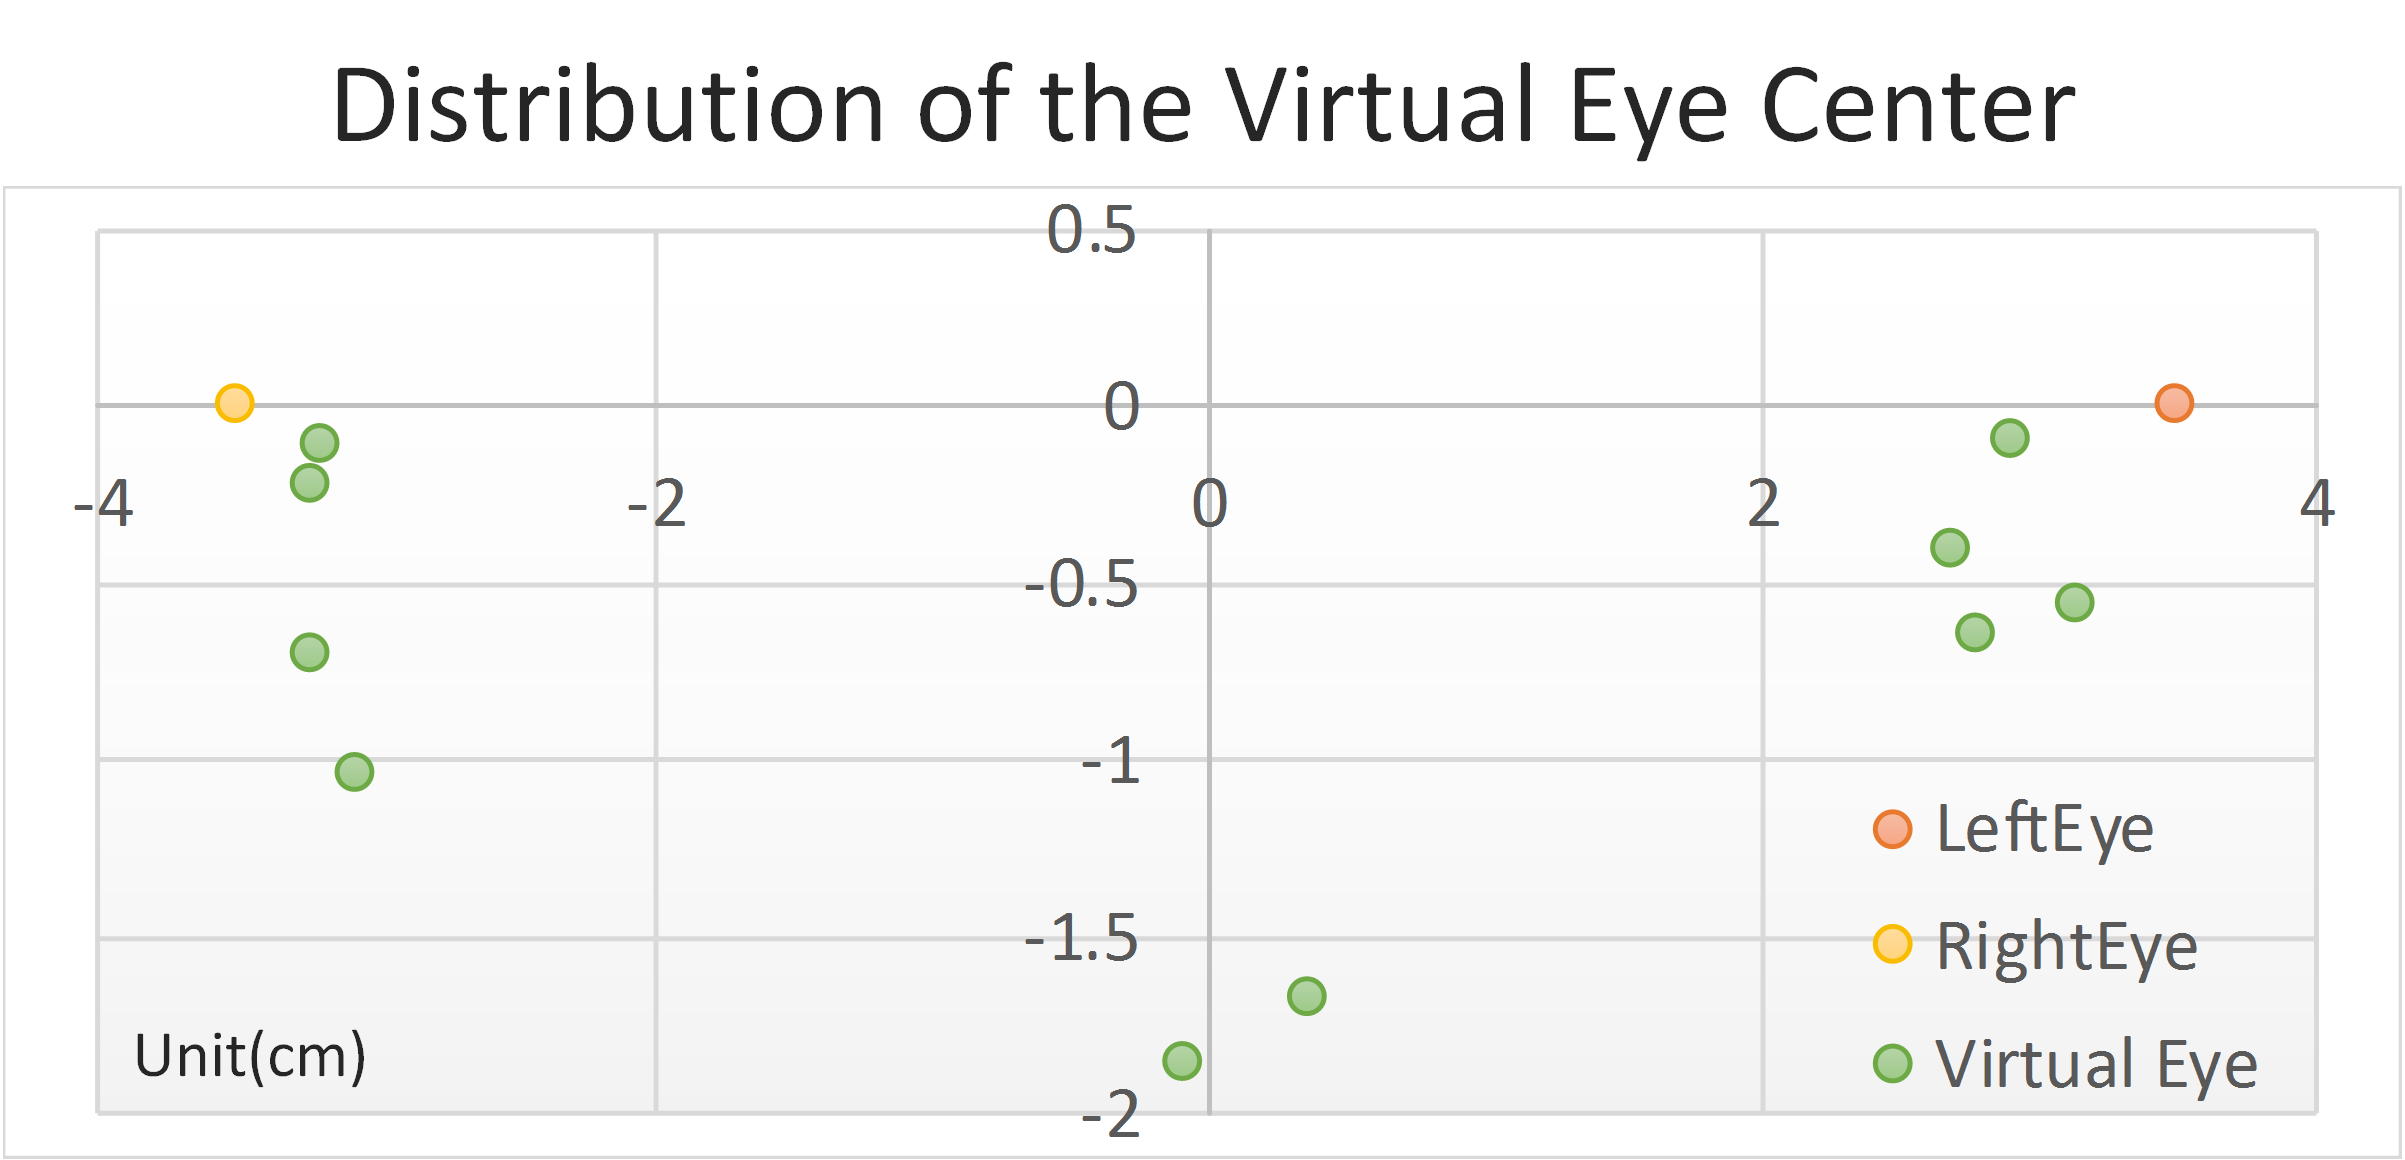
\includegraphics[width=\linewidth]{figures/4-PAST/virtualEye.png}
	\caption{As three points are coplanar, the spatial relationship was shown in a 2D coordinate system. The middle point of the two eyes was set as the original center and the spatial relationship of the left, right and the calculated virtual eye-center is shown in green.}
	\label{fig:4-PAST:virtualEye}
\end{figure}

The average calibration results in step \ref{step:stereoCalib} was taken as the reference to evaluate if the PAST calibration was stable and independent of the distance. The 3D distances from the virtual eye calculated from 1.5, 2, 3, and 4 meters away to the reference one are $0.83\pm0.73cm$, $0.56\pm0.41cm$,$0.90\pm0.73cm$, and $1.02\pm0.72cm$, respectively. 
As shown in \figurename{ \ref{fig:4-PAST:PAST}}, the offset in the XY plane was less than 0.5 cm in most cases. The offset along the Z axis was bigger than the XY plane as the PAST method calculates the intersection of some pointing lines which pass along Z axis. 
%However the offset was still less than 1 cm in most cases.
The 3D distance calculated from 1.5 meters was greater than the one from 2 meters aways, since $\bar\lambda_i$ increases as the $ D_{\bar E2 \bar F_i}$ decreases ( as seen in section \ref{sec:4-PAST:PASTCalibration}).  
The calibrations in 3 and 4 meters were not so stable as the ones in 1.5 and 2 meters as the marker tracking was not so accurate. The four charts in \figurename{ \ref{fig:4-PAST:PAST}} show the PAST method could provide a stable calibration result for different users and the calibration was independent of the contextual environment. 

\begin{figure}[htb]
	\centering
	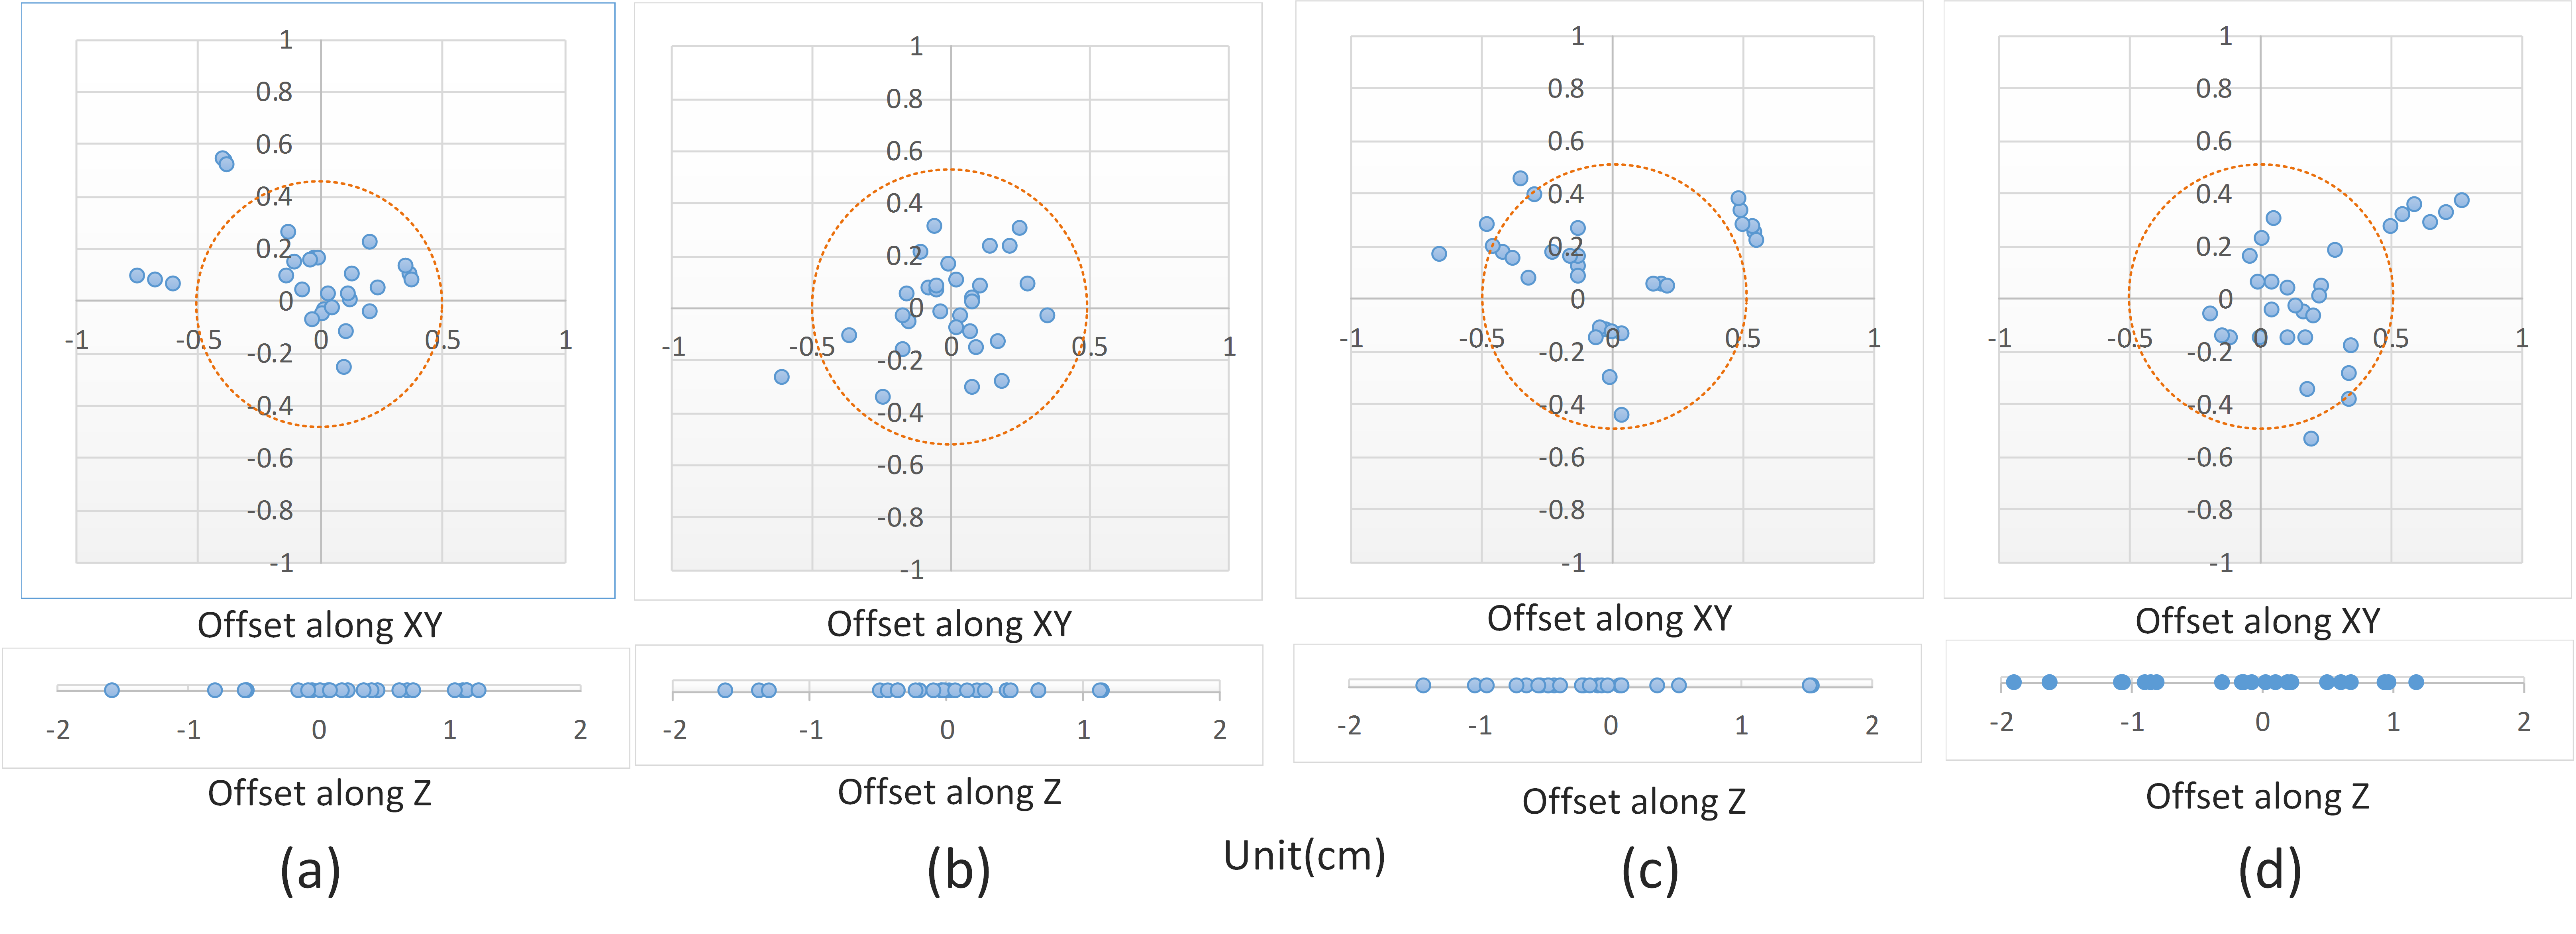
\includegraphics[width=\linewidth]{figures/4-PAST/PAST.png}
	\caption{The calibration results were compared to the reference one showing distribution of the offset along X,Y and Z axis. The XY plane was the one approximately parallel to the user's face. These four charts show the offset of the calibrations from different distances. (a) 1.5 meters away (b) 2 meters away (c) 3 meters away (d) 4 meters away.}
	\label{fig:4-PAST:PAST}
\end{figure}
The first PAST calibration result in step \ref{step:stereoCalib} was employed to evaluate the recovered pointing geometry in different scenarios, with and without visual feedback, with a different hand, from different distance and towards a different display. To evaluate the recovered pointing geometry, ${\angle}_{E}$ was calculated according to Eq. \ref{equ:ViewAngleError} to evaluate the accuracy. The precision was the difference of ${\angle}_{E}$ in consecutive frames while the participant performed pointing gestures to the same target. To get a clear distribution of the error of the recovered pointing lines, the vector from the $\bar T_i$ to $T_i$ was also calculated. As shown in \figurename{ \ref{fig:4-PAST:Accuracy2m}} and \figurename{ \ref{fig:4-PAST:Accuracy}}, for every point in the charts the distance to the original was the angle value in degrees and the points were distributed according to the vector from the $\bar T_i$ to $T_i$.

The pointing accuracies shown in \figurename{ \ref{fig:4-PAST:Accuracy2m}(a-c)} are $0.16\pm0.13$\degree, $0.37\pm0.28$\degree, and $0.60\pm0.73$\degree, respectively.  In \figurename{ \ref{fig:4-PAST:Accuracy2m}(b)} the ${\angle}_{E}$ of most points was less than 0.5\degree (consistent with  \figurename{ \ref{fig:4-PAST:evaluatinOfPointing}} ), so the pointing geometry was correctly recovered. Comparing \figurename{ \ref{fig:Accuracy2m}(a) and \ref{fig:4-PAST:Accuracy2m}(b)}, it was found that the visual feedback improved the accuracy as the user could adjust their pointing gesture. As seen in \figurename{ \ref{fig:4-PAST:Accuracy2m}(c)}, the calibration still worked well with another hand in most cases.The precisions of the pointing line with and without feedback were very stable and less than 0.2\degree, shown in \figurename{ \ref{fig:4-PAST:Accuracy2m}(d)}, so the wearable device could stably recover the pointing geometry.
\begin{figure} [htb]
	\centering
	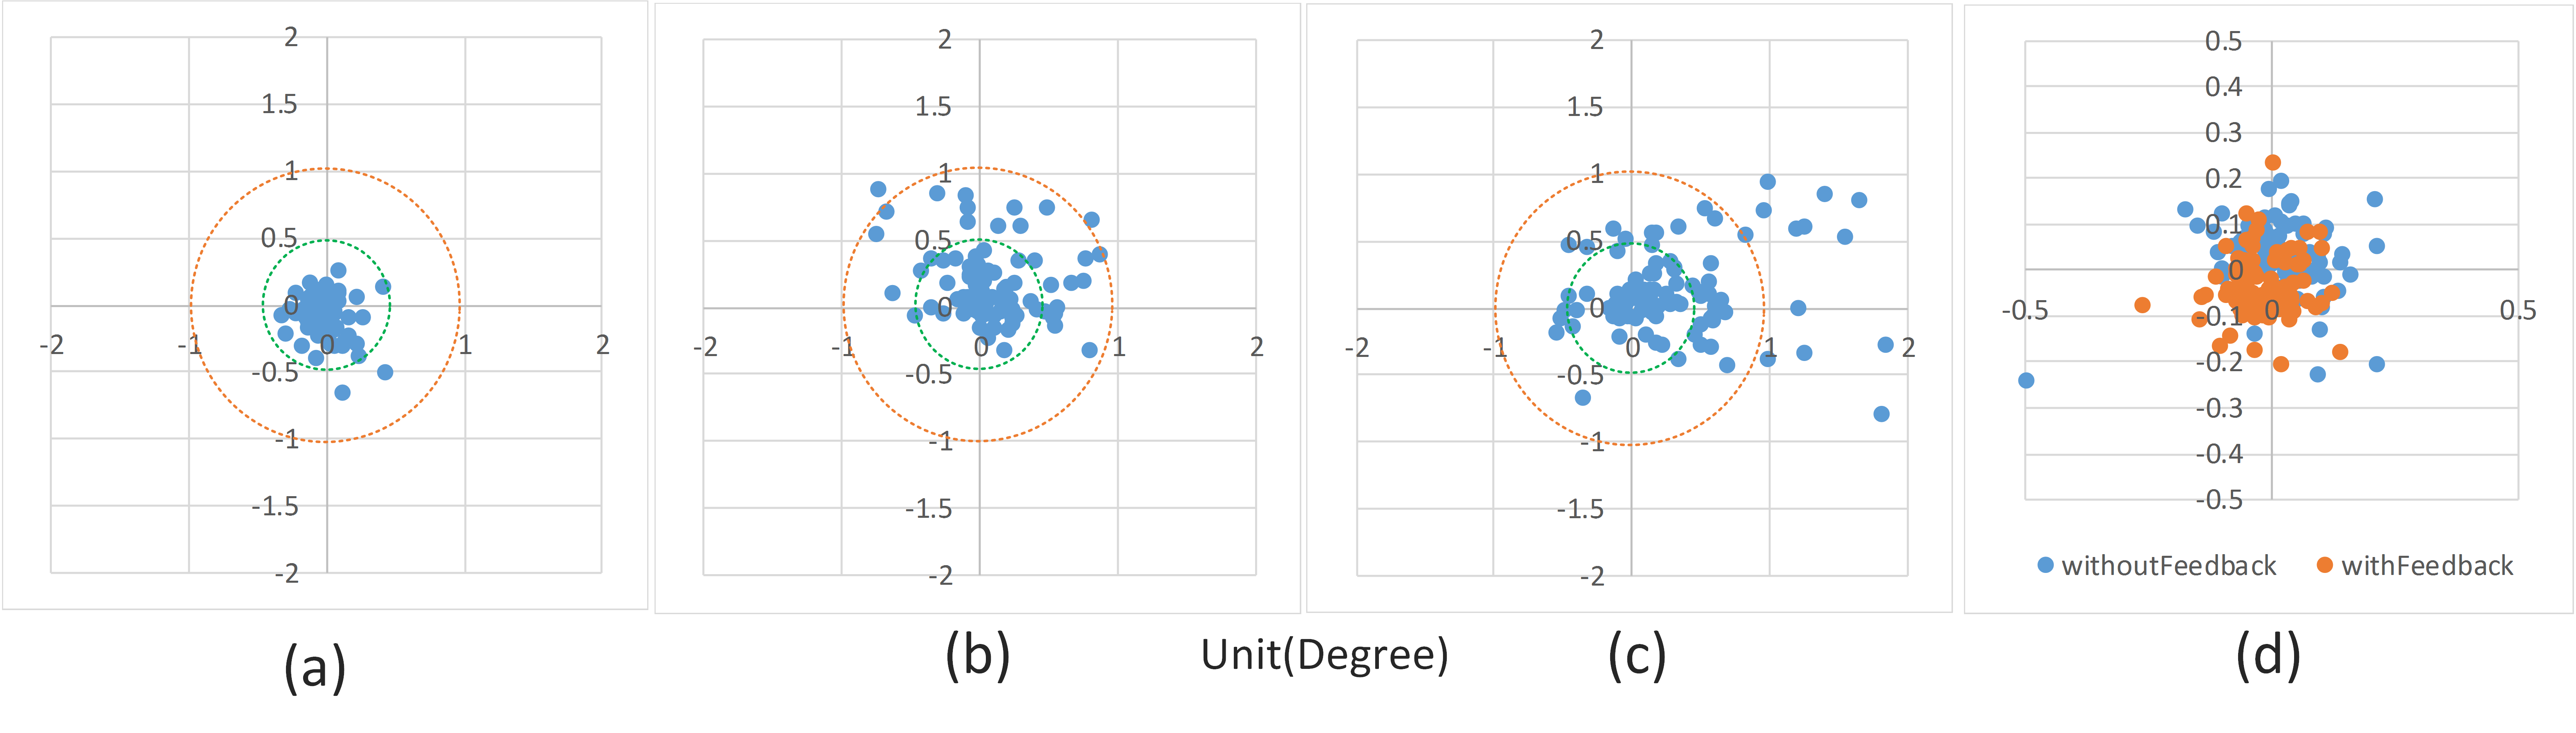
\includegraphics[width=\linewidth]{figures/4-PAST/accuracy2m.png}
	\caption{After calibration, the participants performed pointing gestures towards some targets to evaluate if the pointing geometry could be correctly recovered. (a) perform pointing with feedback from 2 meters away (b) perform pointing from 2 meter aways (c) perform pointing with another hand, different with the one used for calibration (d) the precision when the participants performed pointing with and without feedback from 2 meters away.}
	\label{fig:4-PAST:Accuracy2m}
\end{figure}

The pointing accuracies shown in \figurename{ \ref{fig:4-PAST:Accuracy}(a-d)} are $0.69\pm0.84$\degree, $0.57\pm0.43$\degree, $0.79\pm0.92$\degree, and $0.64\pm0.57$\degree, respectively. As expected in \figurename{ \ref{fig:4-PAST:evaluatinOfPointing}}, the ${\angle}_{E}$ increased at 1.5 meters away in \figurename{ \ref{fig:4-PAST:Accuracy}(a)}, compared to \figurename{ \ref{fig:4-PAST:Accuracy2m}(b)}. However, \figurename{ \ref{fig:4-PAST:Accuracy}(b) and \ref{fig:4-PAST:Accuracy}(c)} show the ${\angle}_{E}$ didn't decrease when the pointing was performed from 3 and 4 meters away as the accuracy of the contextual information declined. \figurename{ \ref{fig:4-PAST:Accuracy}(d)} demonstrates that the calibration was contextually independent and the pointing geometry was still recovered with the 24$''$ monitor. 

As shown in \figurename{ \ref{fig:4-PAST:Accuracy2m}} and \figurename{ \ref{fig:4-PAST:Accuracy}}, ${\angle}_{E}$ is less than 1\degree in most cases in different scenarios and less than 0.5\degree with an accurate contextual information. The overall pointing accuracy at 1.5, 2, 3, and 4 meters is $0.60\pm0.70$\degree. We conclude that the pointing gesture was recovered accurately.
\begin{figure} [htb]
	\centering
	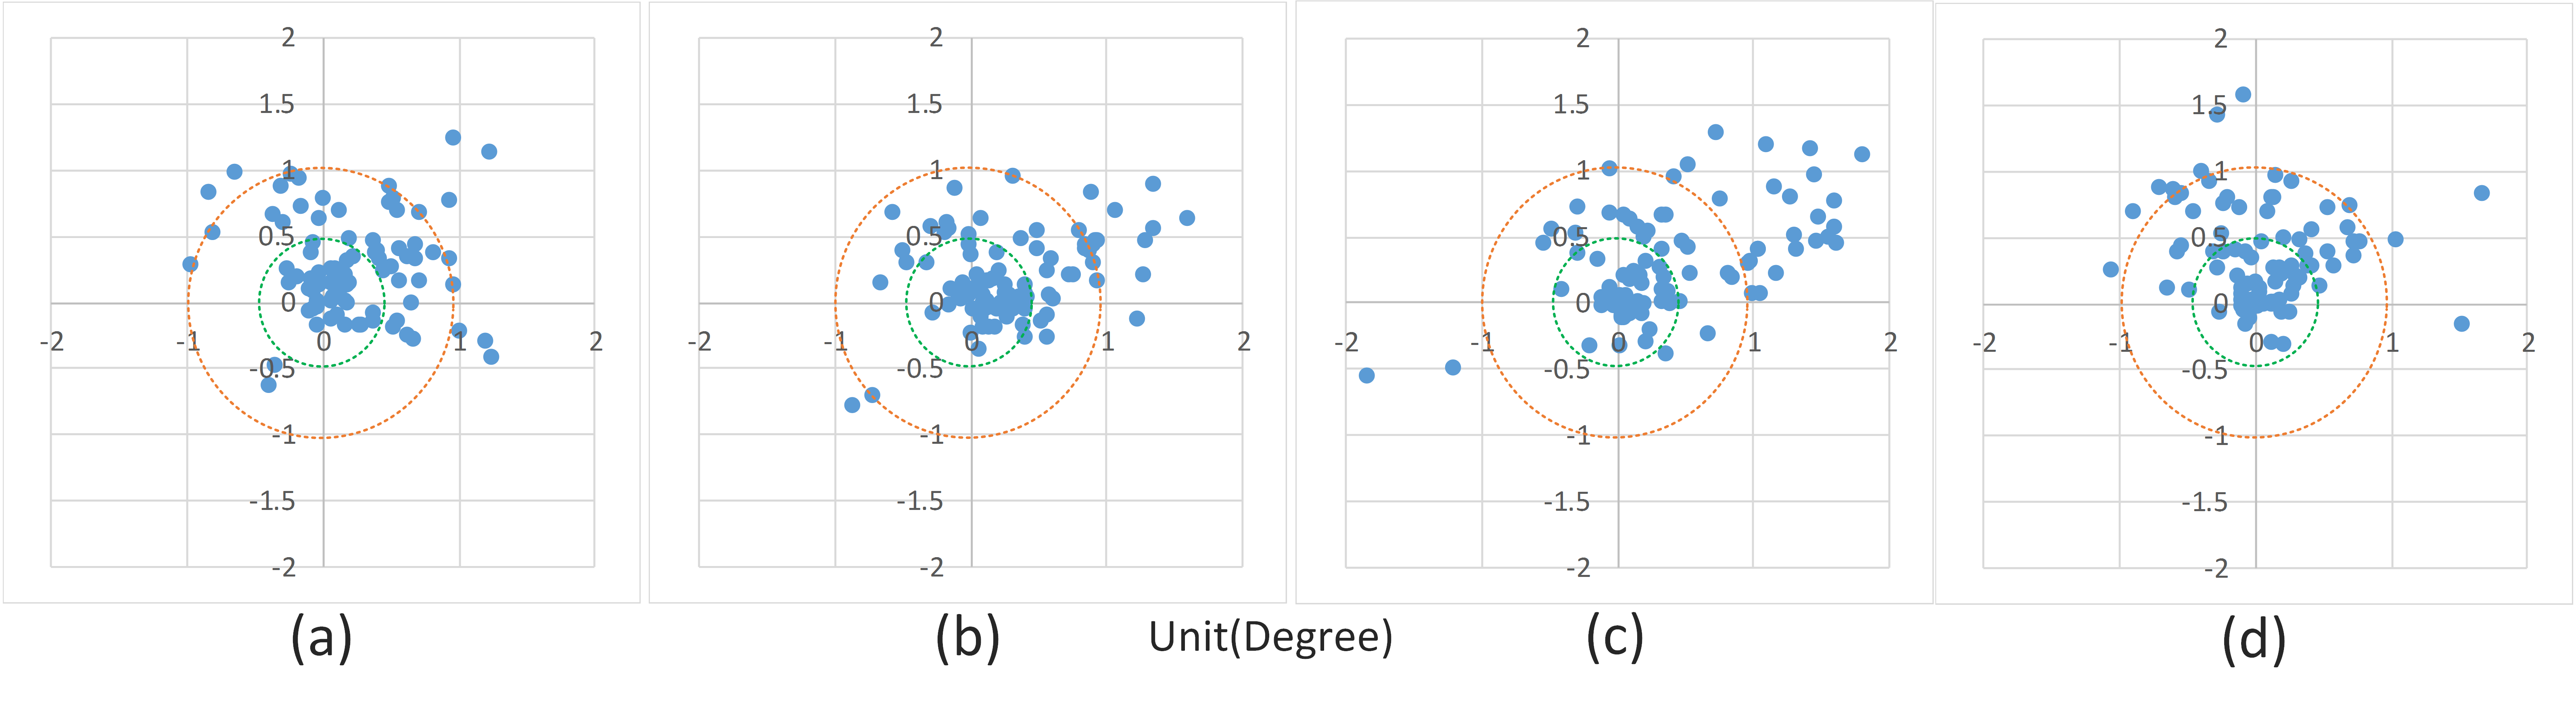
\includegraphics[width=\linewidth]{figures/4-PAST/accuracy.png}
	\caption{The participants performed pointing gesture towards some targets in different scenarios to evaluate if calibration was contextually independent. (a) perform pointing from 1.5 meters away (b) 3 meters away (c) 4 meters away (d) perform pointing towards the 24 in monitor }
	\label{fig:4-PAST:Accuracy}
\end{figure}

%questionnaire
A questionnaire was designed to get a qualitative evaluation about the pointing interaction and the ``PictureView" demo. A Likert scale was used which is a type of psychometric response scale often used in surveys and is the most widely used scale in survey research. When responding to a Likert questionnaire item, participants specify their level of agreement to a statement. The format of our 5-pt Likert was: (1) strongly disagree, (2) disagree, (3) neither agree nor disagree, (4) agree, (5) strongly agree.
\begin{table}
	\caption{The Likert scale results of the questionnaire}
	\label{tb:4-PAST:questionnaire}
	\scriptsize
	\begin{center}
		\begin{tabular}{p{5.5cm}|p{1.2cm}}
			Questions & Scale \\
			\hline
			\textit{Q1:}I think that I would like to use this system &  $4.0\pm0.8$ \\
			\textit{Q2:}I found the system necessarily complex & $4.7\pm0.5$ \\
			\textit{Q3:}I thought the system was easy to use & $4.2\pm0.9$ \\
			\textit{Q4:}I don't think that I would need the support of a technical person to be able to use this system & $4.1\pm1.0$\\
			\textit{Q5:}I  think the system is consistent & $4.3\pm0.6$ \\
			\textit{Q6:}I would imagine that most people would learn to use this system very quickly & $4.4\pm0.5$ \\
			\textit{Q7:}I felt very confident using the system & $4.3\pm0.6$ \\
			\textit{Q8:}I didn't need to learn a lot of things before I could get going with this system & $4.5\pm0.5$
		\end{tabular}
	\end{center}
\end{table}
As shown in table \ref{tb:4-PAST:questionnaire}, all questions attained a positive scores above 4.0. Q1 had the lowest score as some participants felt a little tired while continuously lifting their arm to perform pointing gestures. In the demo the selection command was recognized as the user pushed their fingers along the pointing line, which was a little different than with a natural click hand gesture, thus the participant required some time to get used to it. In general the participants liked the pointing interaction very much and could learn it very easily and quickly. In their opinion, the finger pointing interaction was very natural. 

\subsection{Discussion \& Conclusion}
PAST offers a novel concept and method for recovering the user specific pointing habits that enables direct interaction with real and virtual digital elements of interest within the user's environment. 
As seen in \figurename{ \ref{fig:4-PAST:virtualEye}}, the virtual eye center $E$ calculated by PAST is user specific. The PAST calibration is very important for recovering the user specific pointing geometry. In addition, the proposed method is contextually independent and could also be used to calculate the eye position in the wearable device coordinate system. 

As shown in our user study, the PAST method could finish calibration stably and recover the user specific pointing geometry in different scenarios, with an accuracy of less than $0.5\degree$ with an accurate contextual information and less than $1\degree$ in most cases. The participants could easily learn how to use this new interaction method. However, the gesture combined with the pointing still should be improved. In addition, the PAST calibration could be separately done for every  finger allowing the user to use multi-finger to perform a multi-control 3D interaction in a mixed reality setting. Given the recent increased interest in using speech to interact with mobile devices, it is a logical next step to support a user in pointing at an object while stating a comment or asking a question about it.

Pointing At Several Targets method facilitates the calibration of the user's pointing gesture that models and recovers the user specific pointing geometry and subsequently calculates where the user is pointing at. Mathematical analysis and experimental results demonstrate that the PAST method could model and calibrate the pointing gesture stably and recover the user specific pointing gesture correctly. The calibration method is contextually independent and in most cases the pointing line was recovered with accuracy less than $1\degree$ and less than $0.5\degree$ with accurate contextual information. The overall pointing accuracy at 1.5, 2, 3, and 4 meters is $0.60\pm0.70$\degree. The PAST solution would enable a whole series of applications in which the user may acquire or interact with digital information and opens the path towards development of new interaction paradigms: the user could directly perform multi-control 3D interaction with virtual or real elements placed within the mixed reality environment.